\chapter{Identification and tuning of the controllers}\label{ch:tuning}
In this chapter we will look at the tuning of the different controllers of the system. Firstly we will look at the secondary controllers, before we later move on to the higher level controlllers. A summary of the different controller parameters can be found in \autoref{table:controllerparam}.

\begin{table}[h]
	\caption{Summary of controller parameters in the plant}
	\label{table:controllerparam}
	\begin{center}
	\begin{tabular}{|c|c|c|c|}
	\hline
	Controller & $K_p$ & $T_i$ & $G$ \\
	\hline
	\texttt{24\_FC1005} & $1.18125$ & $5$ & $1.72$ \\
	\texttt{24\_FC1015} & $0.2$ & $5$ & $1.28$\\
	\texttt{24\_FC1019} & $0.27225$ & $5$ & $0.41$ \\
	\texttt{24\_LC1015} & $9.66$ & $1200$ & $-3.22$ \\
	\texttt{24\_LC1016} & $3.3$ & $750$ & $-0.89$ \\
	\texttt{24\_LC1028} & $47.9$ & $128$ & $-1.13$ \\
	\texttt{24\_PC1024} & $17.5$ & $2400$ & $-1.62$\\
	\texttt{24\_TC1015} & $66$ & $1440$ & $-0.44$\\
	\texttt{24\_TC1088} &$5.02$ & $1440$ & $-0.49$\\
	\hline
	\end{tabular}
	\end{center}
\end{table}

\section{Tuning of secondary controllers}\label{sec:tuning_secondary}
Firstly we want to tune the secondary controllers, which do not depend much on which control structure is used for composition control. The controllers this applies to is the flow controllers \texttt{24\_FC1005}, \texttt{24\_FC1015} and \texttt{24\_FC1019}, the level controller \texttt{24\_LC1028}, and also the pressure controller \texttt{24\_PC1024}. These controllers all have fast dynamics compared to the composition control and primary level controllers.

\subsection{Tuning of \texttt{24\_FC1019}}
Firstly we tune the controller \texttt{24\_FC1019}, which is a flow controller controlling the bottom flow $B$ of N-butane. When trying to apply Skogestad IMC-tuning to a first order model, the results were poor as there are close to none time delay, as expected in a valve, which lead to this being a unprecise model. Ziegler-Nichols method, as described in \cite{balchen2003reguleringsteknikk}, was then a natural choice, and with a critical gain of $K_{p_k} = 0.605$ and integral time $T_i \to\infty$ we got the osciallations shown in \autoref{fig:fc1019_oscillations}. By zooming into this we read the period of the oscillations as $T_k = \SI{6}{\second}$. This yields the gain and integral time $K_p = 0.27225$ and $T_i = \SI{5}{\second}$. With this tuning we get the response shown in \autoref{fig:fc1019_tuned}. This is a good response to a relatively large step reference change. Before the reference step the controller has an external set point, that is why the set point is changing dynamically. When doing the step change, the controller settings was changed from external to internal set point, and then back to external for the second step.

\begin{figure}[ht!]
	\centering
	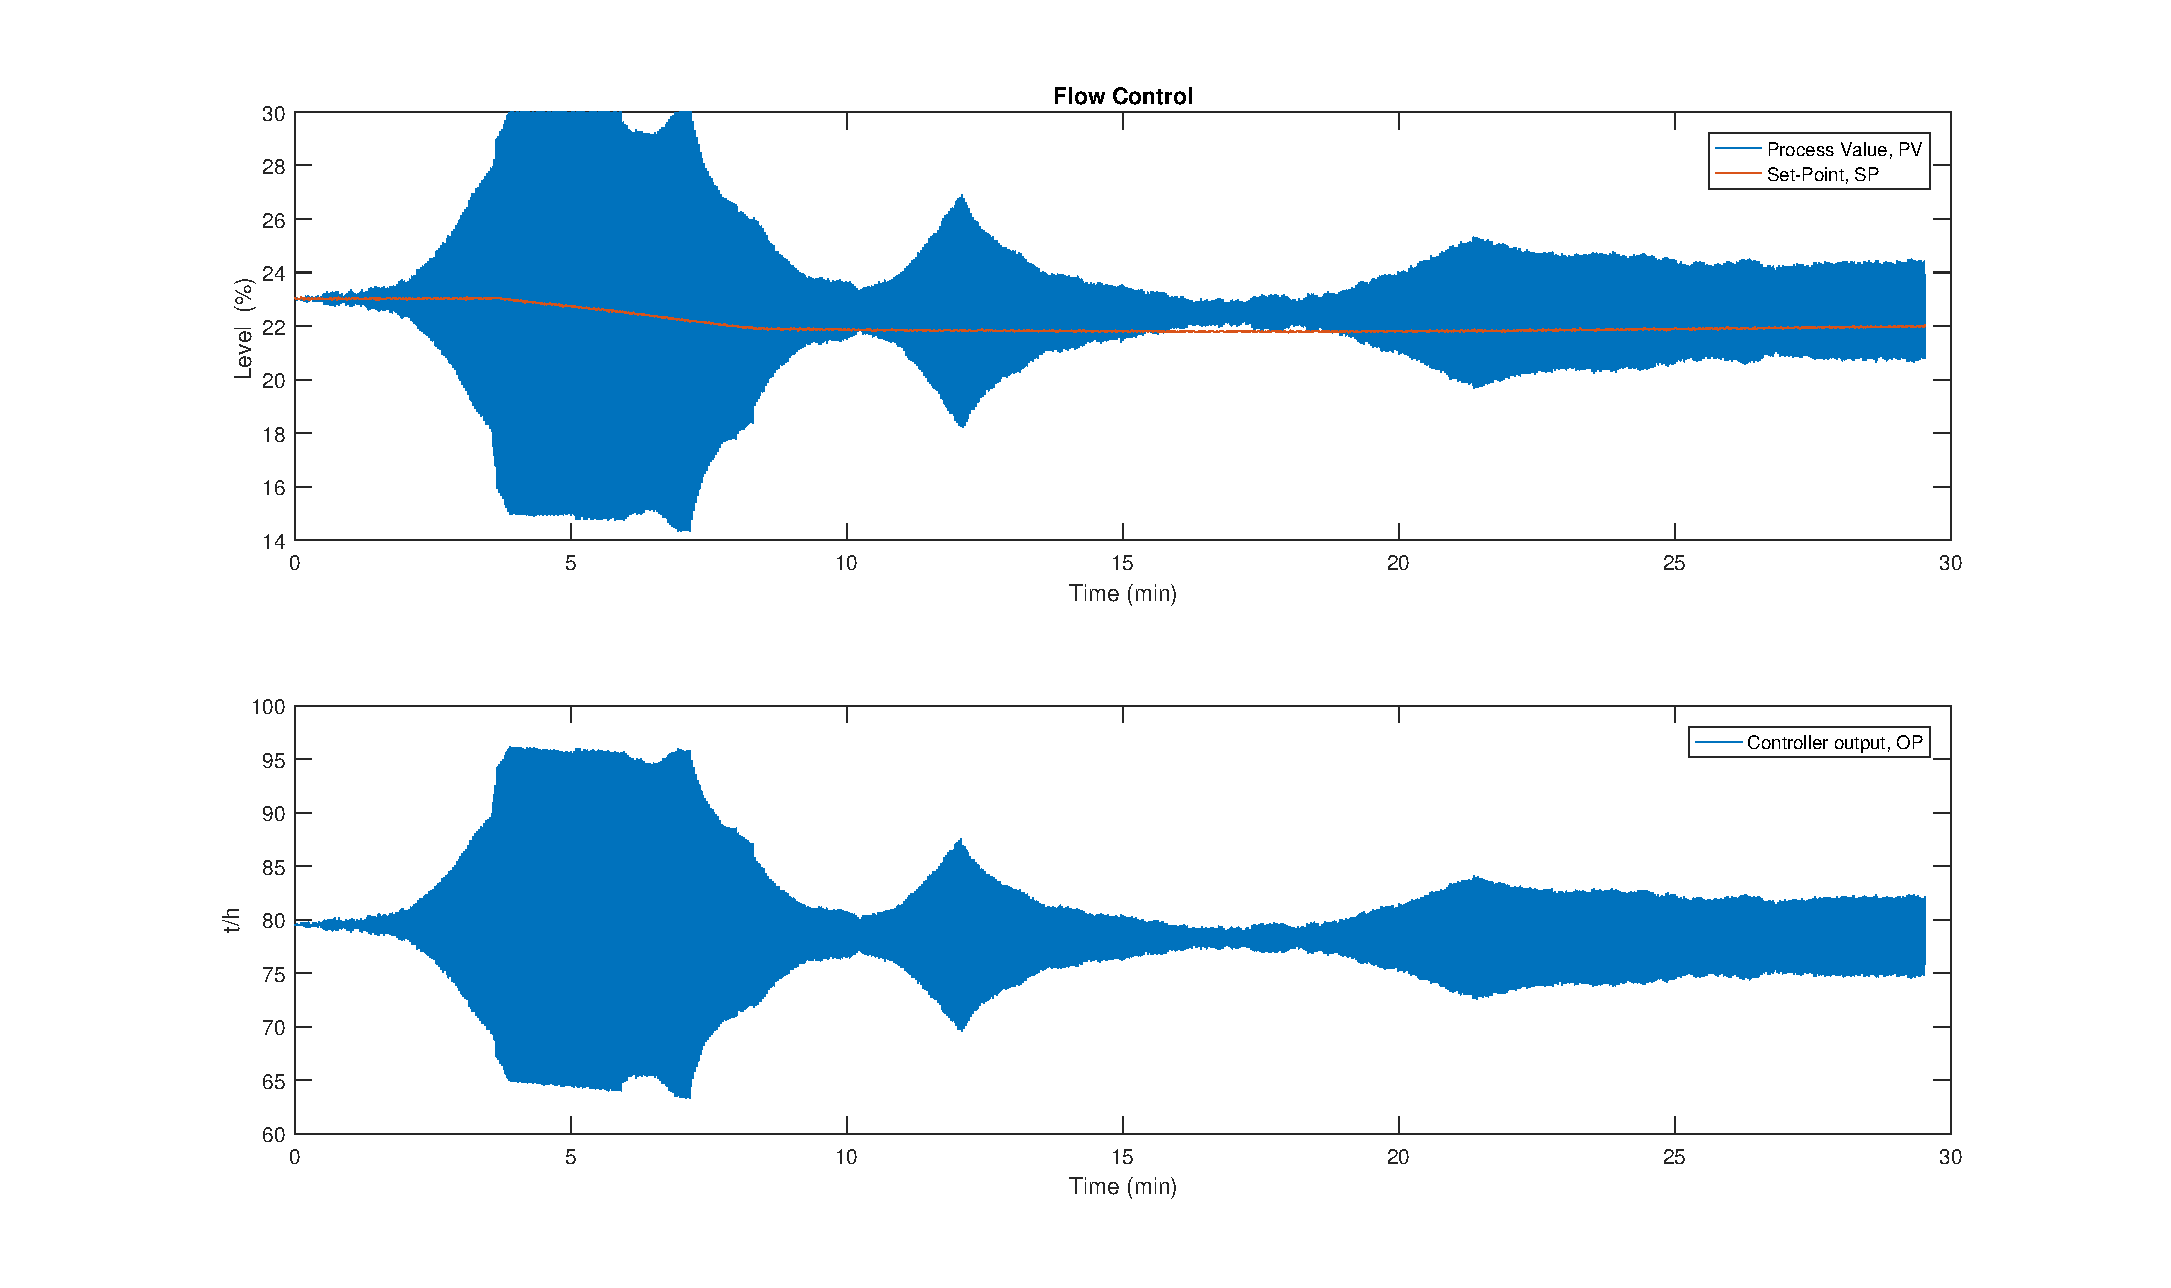
\includegraphics[width=0.85\textwidth]{fig/tuning/FC1019_critical.eps}
	\caption{Oscillations of the flow controller \texttt{24\_FC1019} with $K_{p_k} = 0.605$ from about $\SI{22}{\minute}$}
	\label{fig:fc1019_oscillations}
\end{figure}

\begin{figure}[ht!]
	\centering
	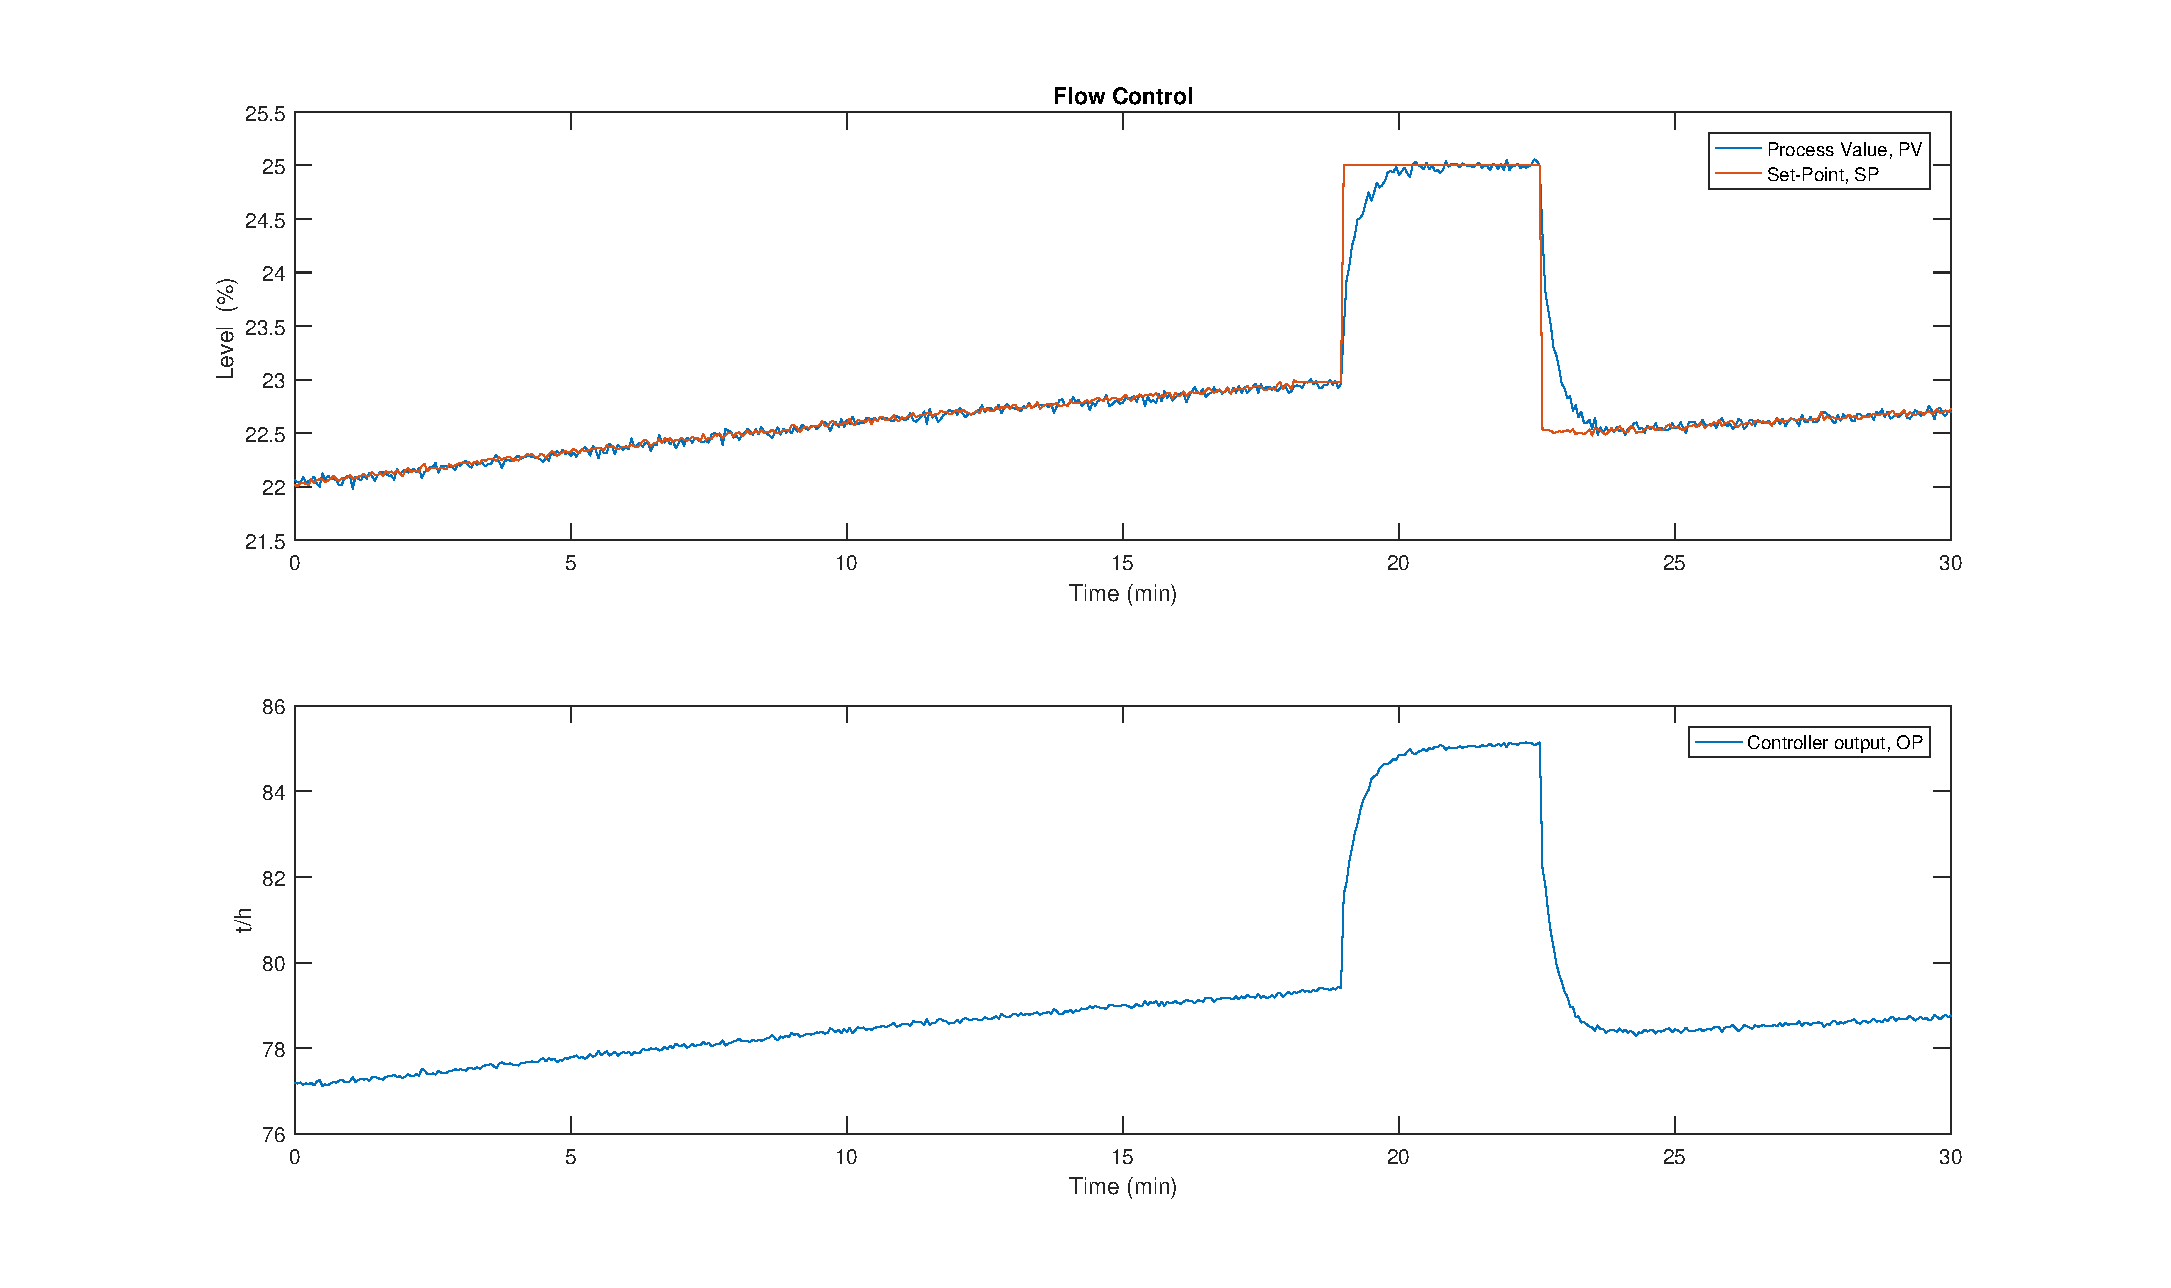
\includegraphics[width=0.85\textwidth]{fig/tuning/FC1019_tuned.eps}
	\caption{Response of \texttt{24\_FC1019} tuned using Ziegler-Nichols method}
	\label{fig:fc1019_tuned}
\end{figure}

\subsection{Tuning of \texttt{24\_FC1005}}
We now tune the controller \texttt{24\_FC1005}, another flow controller, this one controlling $D$, the distillate flow of Iso-butane. Using the same method as in the tuning of \texttt{24\_FC1019}, we find the critical values $K_{p_k} = 2.625$ and $T_k = 6 \si{\second}$. This yields the parameters $K_p = 1.18125$ and $T_i = 5 \si{\second}$. As we see in \autoref{fig:fc1005_tuned}, the we get a slow oscillation when switching back to external reference, but this is due to oscillations in the set point, and not the process value. We see that the process nicely follows the reference with high accuracy.

\begin{figure}[ht!]
	\centering
	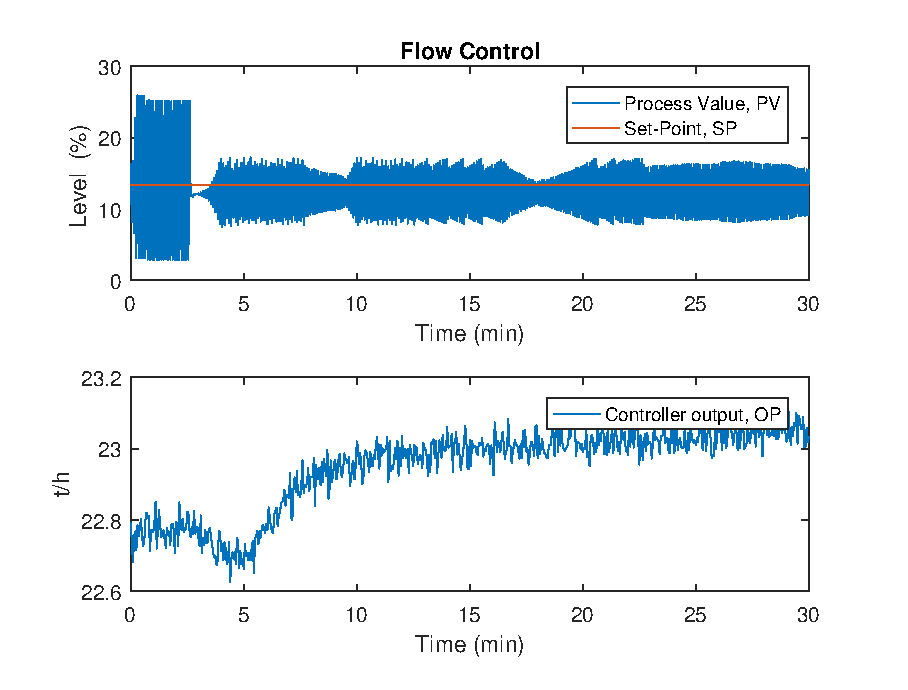
\includegraphics[width=0.85\textwidth]{fig/tuning/FC1005_critical.eps}
	\caption{Oscillations of the flow controller \texttt{24\_FC1005} with critical gain $K_{p_k} = 2.625$ from about $\SI{23}{\min}$}
	\label{fig:fc1005_oscillations}
\end{figure}

\begin{figure}[ht!]
	\centering
	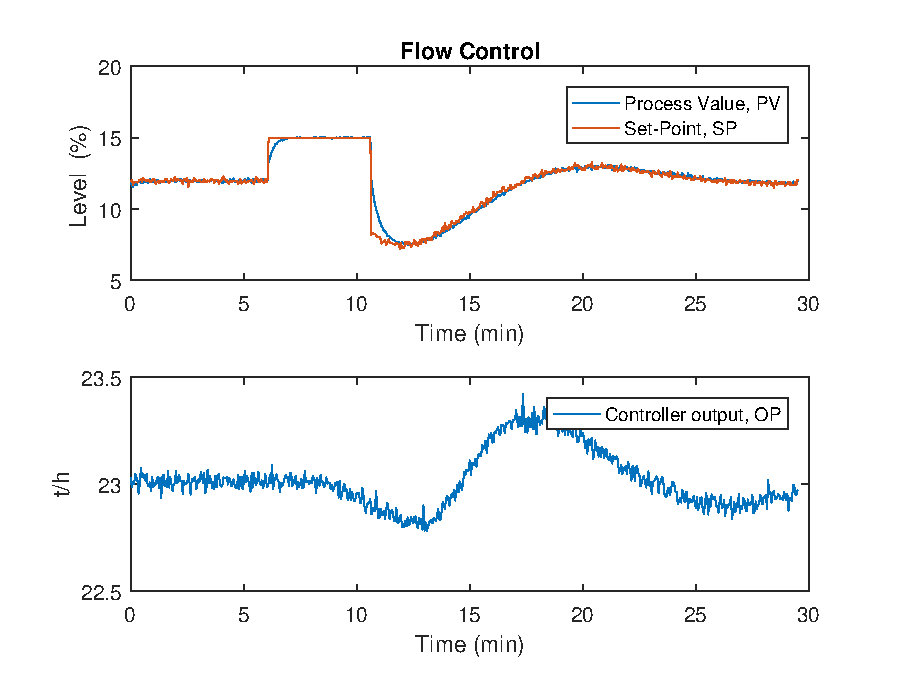
\includegraphics[width=0.85\textwidth]{fig/tuning/FC1005_tuned.eps}
	\caption{Response of \texttt{FC\_1005} tuned using Ziegler-Nichols method}
	\label{fig:fc1005_tuned}
\end{figure}

\subsection{Tuning of \texttt{24\_LC1028}}
Further we tune the level controller \texttt{24\_LC1028} wich controls the area for heat exhange in the bottom heat exchanger. This makes it indirectly control the bottom vapour flowrate $V$. Here we use the SIMC-method for tuning of PI(D)-controllers. Using this method we now need to take into account the internal scaling in the controller. By setting the integral time $T_i \to\infty$ we get a simple P-controller which we apply a step in the reference. By using the SIMC-tuning rules from \cite{skogestad2005multivariable} applied on a integrating step response we get

\begin{equation}\label{eq:simc}
	\begin{aligned}
		k' &= \frac{\Delta y}{\Delta t \Delta u}\\
		K_c &= \frac{1}{k'}\frac{1}{\tau_c + \theta} \\
		T_i &= 4(\tau_c + \theta)
	\end{aligned}
\end{equation}

where $\tau_c$ is chosen as $3\theta$ to achieve robustness. Smaller $\tau_c$ improves preformance, but makes the system less robust, as described in \cite{skogestad2005multivariable}. By measuring on \autoref{fig:lc1028_simc} we get the observations

\begin{equation}
	\begin{aligned}
		\Delta u &= 1\\
		\Delta y &= -0.3413\\
		\Delta t &= 462 \\
		\theta &= 8\\
	\end{aligned}
\end{equation}
which again gives the results

\begin{equation}
	\begin{aligned}
		K_c &= -42.3\\
		T_i &= 128\\
	\end{aligned}
\end{equation}

The scaling factor can be calculated as shown in \eqref{eq:scaling}, and when applying a step input with $\Delta y_{\text{ref}} = 2$, we get the immediate response $\Delta u_{\text{meas}} = -17.68$. $\Delta u_\text{exp} = K_p\Delta y_{\text{ref}} = 20$, which gives the scaling factor
\begin{equation}
	G = \frac{u_{\text{exp}}}{u_{\text{meas}}} = -1.13
\end{equation}
which again gives the controller parameters

\begin{equation}
	\begin{aligned}
		K_{p,\text{applied}} &= GK_c = 47.9\\
		T_i &= 128
	\end{aligned}
\end{equation}

This again leads to fairly good response, although the controller is maybe slightly aggressive. This is shown in \autoref{fig:lc1028_tuned}. The equations for the scaling parameter are given as

\begin{equation}\label{eq:scaling}
	\begin{aligned}
		\Delta u_{\text{exp}} &= K_p \Delta y_{\text{ref}} \\
		G &= \frac{\Delta u_{\text{exp}}}{\Delta u_{\text{meas}}} \\
		\implies K_{p,\text{applied}} &= GK_p
	\end{aligned}
\end{equation}


\begin{figure}[ht!]
	\centering
	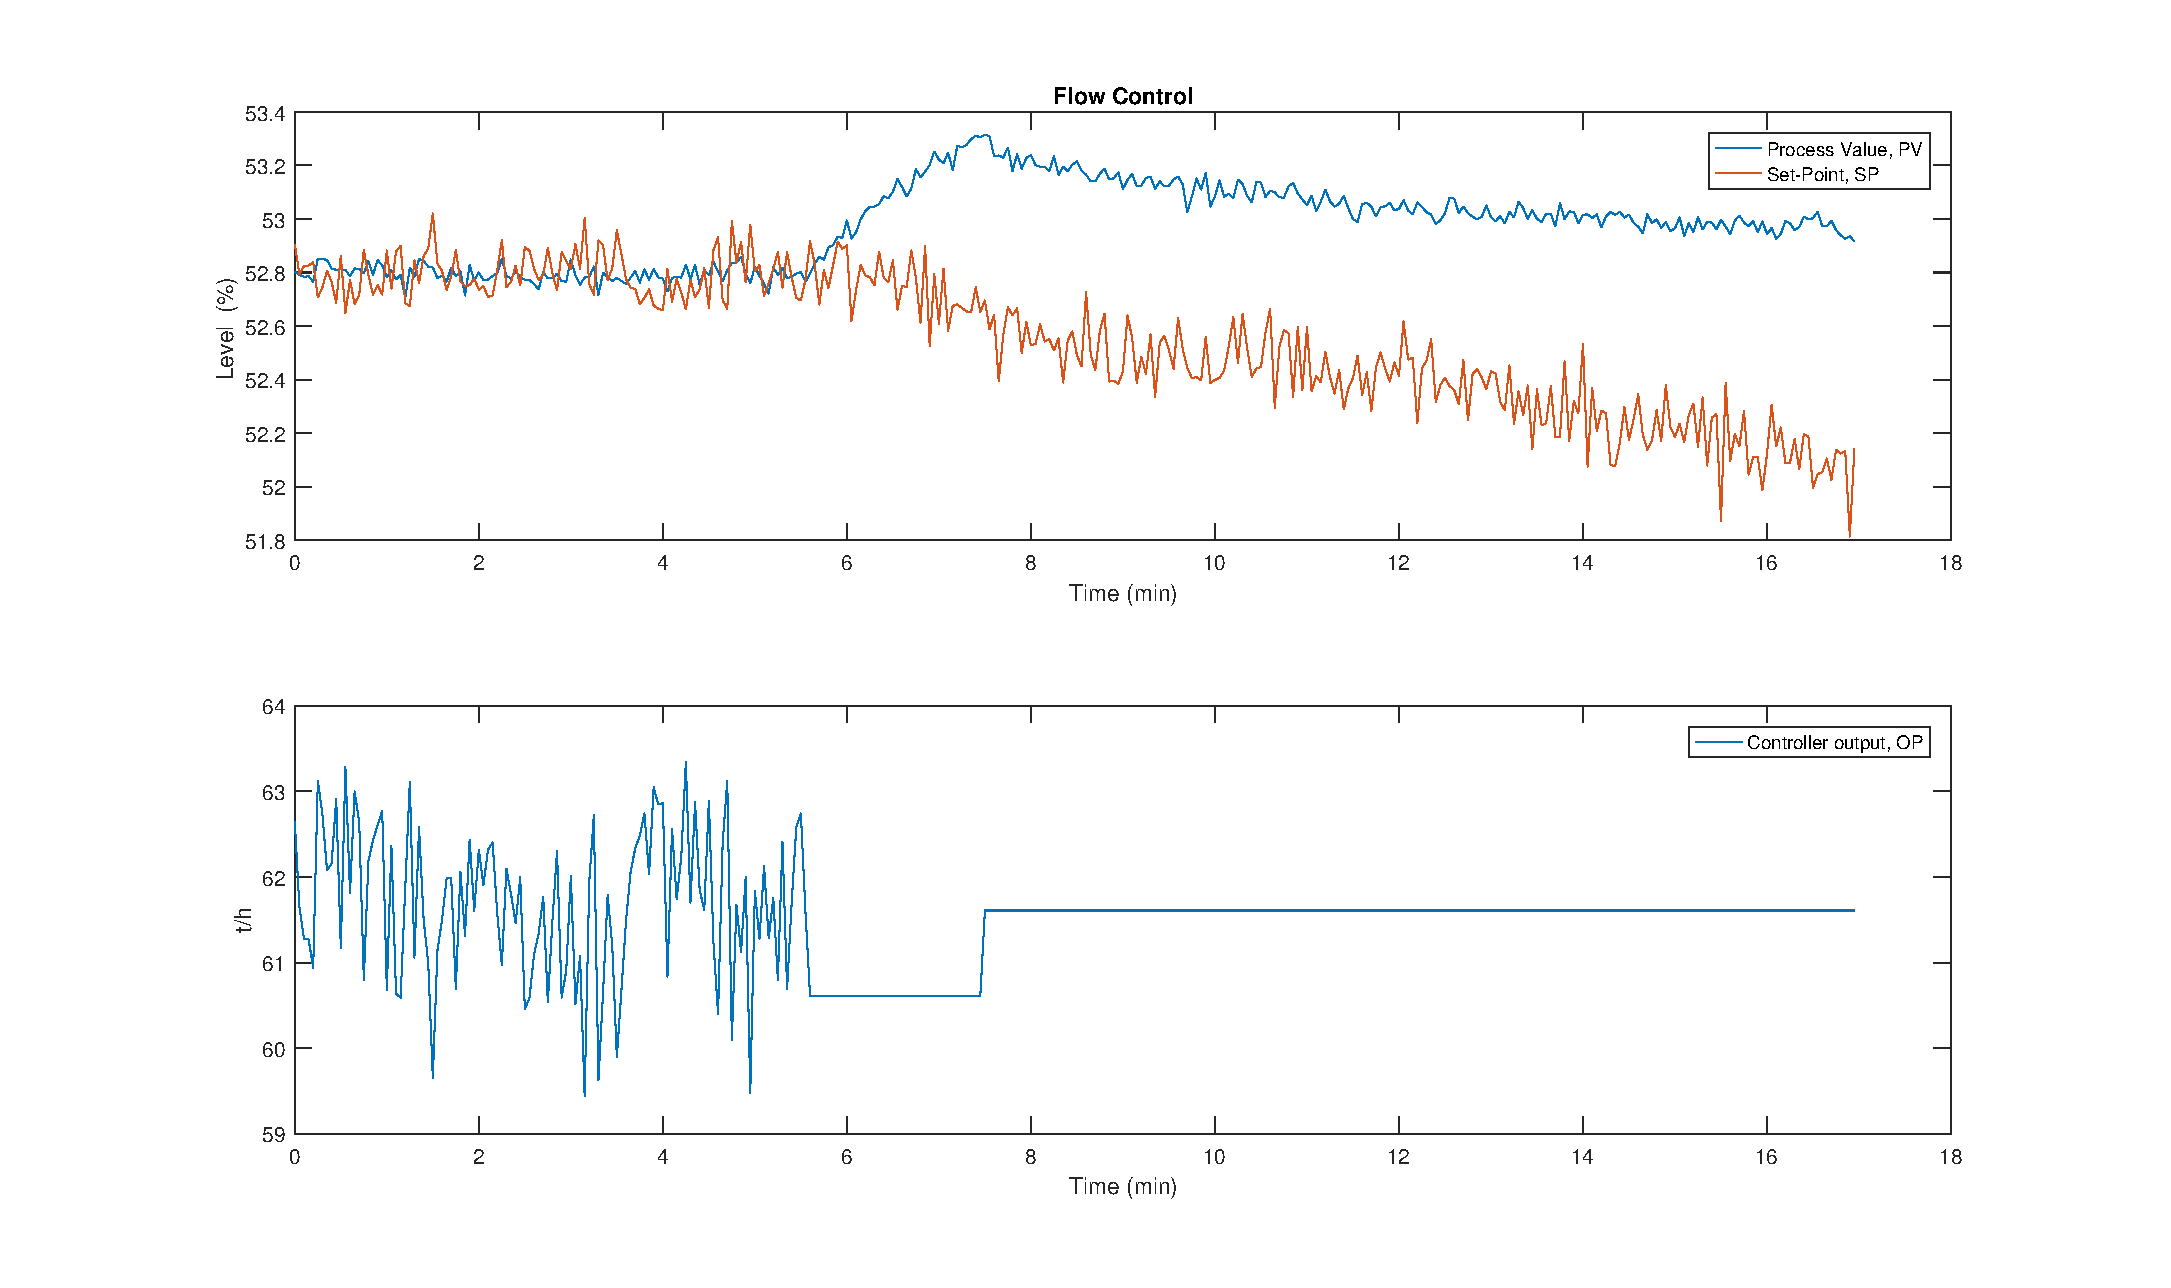
\includegraphics[width=0.85\textwidth]{fig/tuning/LC1028_simc.eps}
	\caption{Output of \texttt{24\_LC1028} with simple P-controller and applied step at $t \approx \SI{7}{\minute}$}
	\label{fig:lc1028_simc}
\end{figure}

\begin{figure}[ht!]
	\centering
	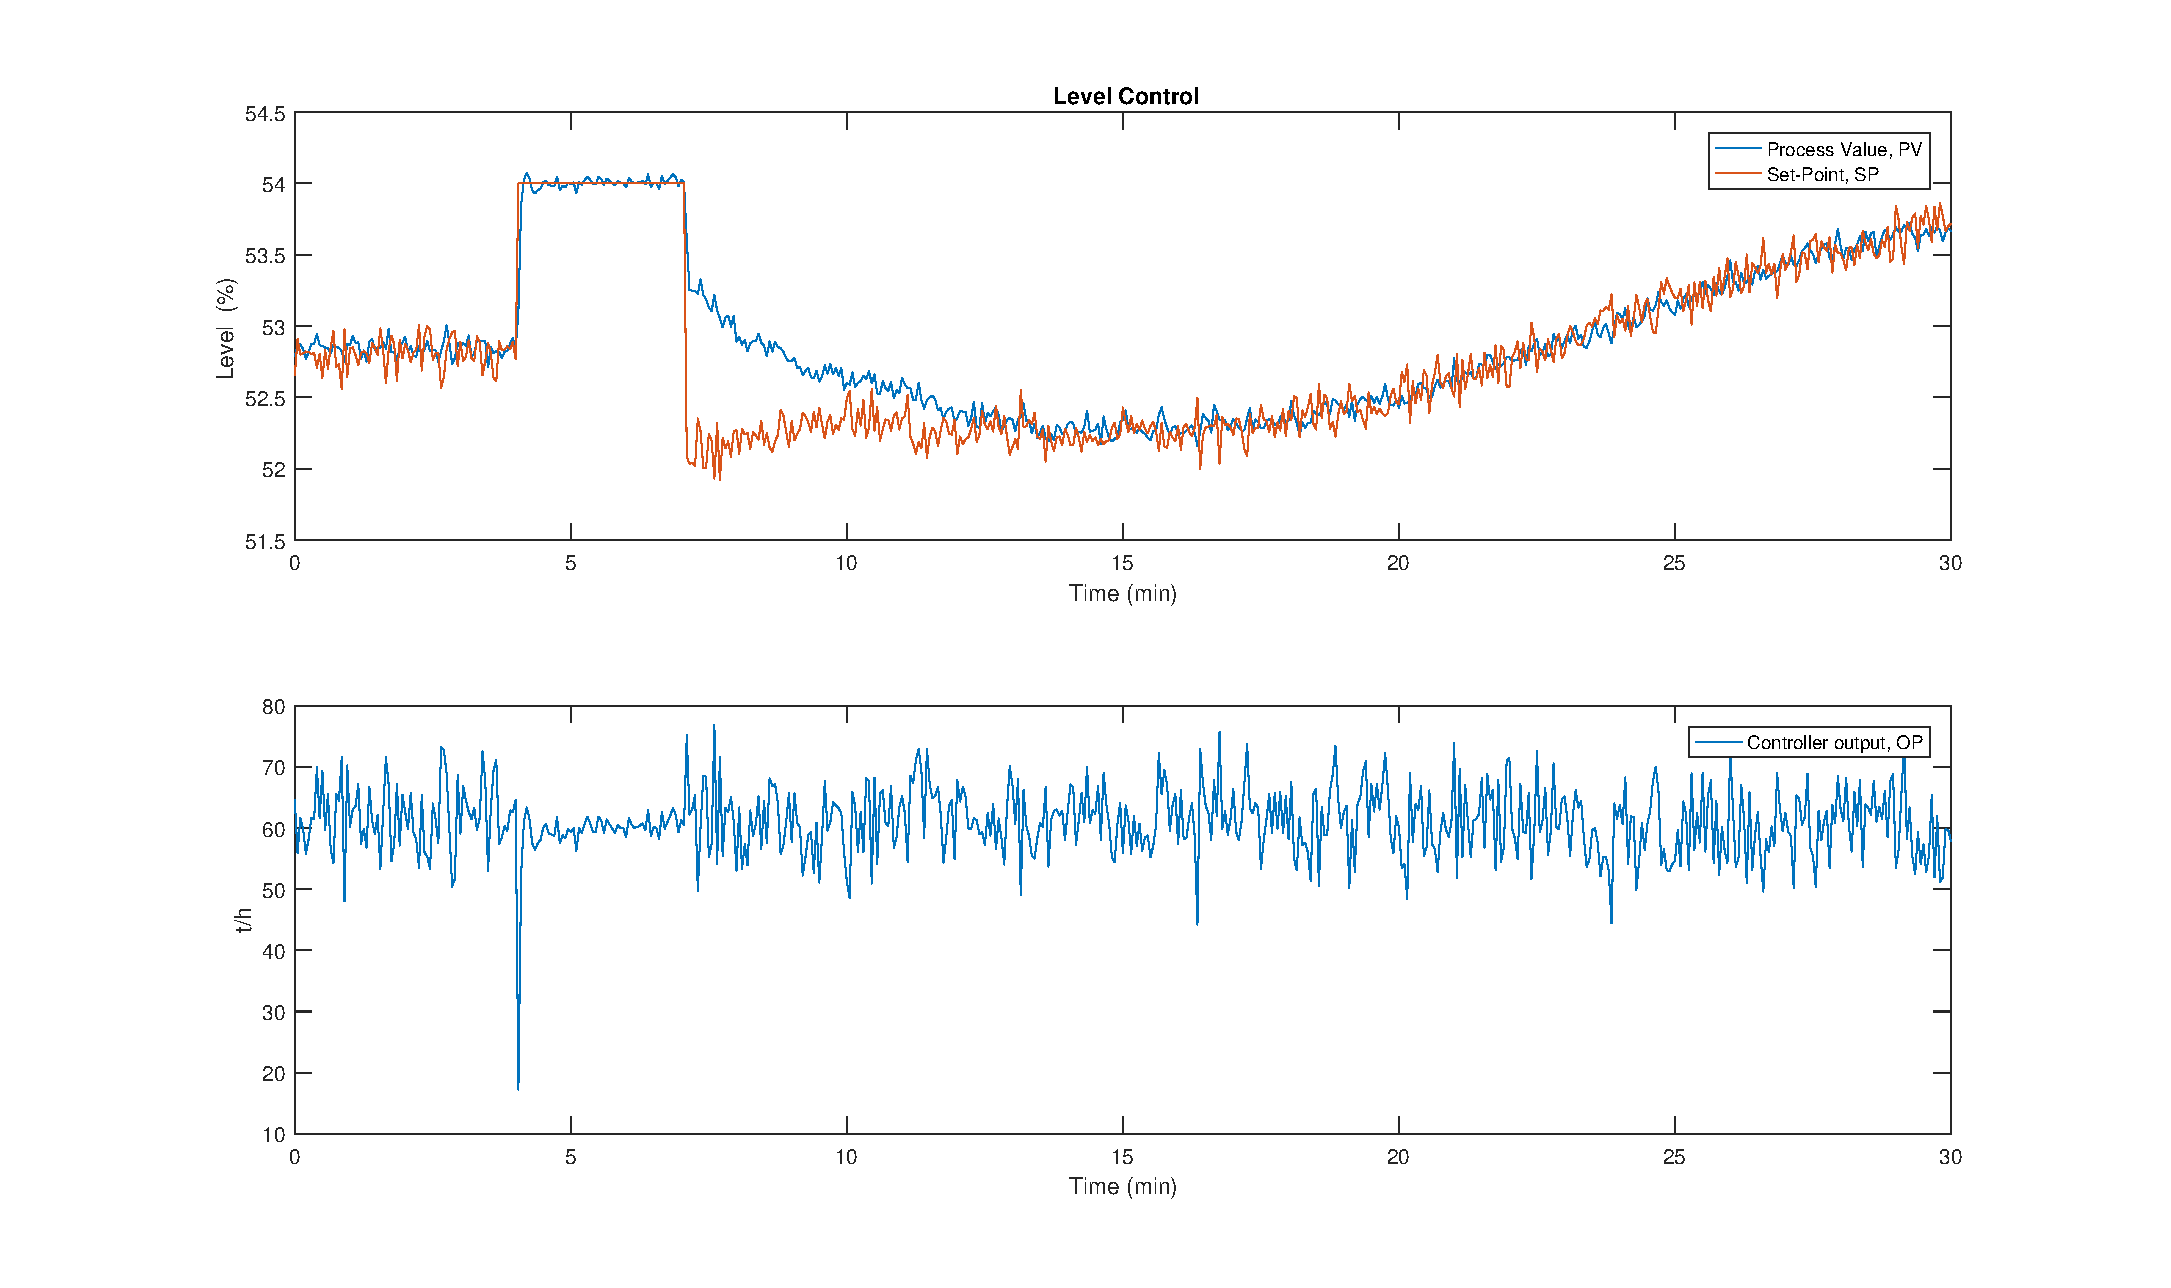
\includegraphics[width=0.85\textwidth]{fig/tuning/LC1028_tuned.eps}
	\caption{Output of \texttt{24\_LC1028} tuned using SIMC and PID-scaling}
	\label{fig:lc1028_tuned}
\end{figure}


\subsection{Tuning of \texttt{24\_PC1024}}
When applying a step oon the input of the pressure controller \texttt{PC\_1024} we get the output response shown in \autoref{fig:pc1024_simc}. When then applying the SIMC method to this output response, we see that we do not have a proper first order model with delay or a clean integrating response with delay, we instead treat the time from the step until the integration starts properly as the time delay $\theta$. We also calculate the internal gain as in \eqref{eq:scaling} and obtain the parameters $G = -1.62$, $\delta u = 0.3$, $\delta t = 900$, $\delta y = -0.021$ and $\theta = 300$. Using the rules from \eqref{eq:simc} and chosing $\tau_c = \theta$ for faster control we get the controller parameters

\begin{equation}
	\begin{aligned}
		K_p &= GK_c = 17.5\\
		T_i &= 4(\tau_c + \theta) = 2400
	\end{aligned}
\end{equation}
This integral time seems quite large, but when looking at the response of the \texttt{PC\_1024} after tuning the parameters, shown in \autoref{fig:pc1024_tuned}, we see that the controller response is fairly good, and keeps the pressure well within acceptable deviations.

\begin{figure}[ht!]
	\centering
	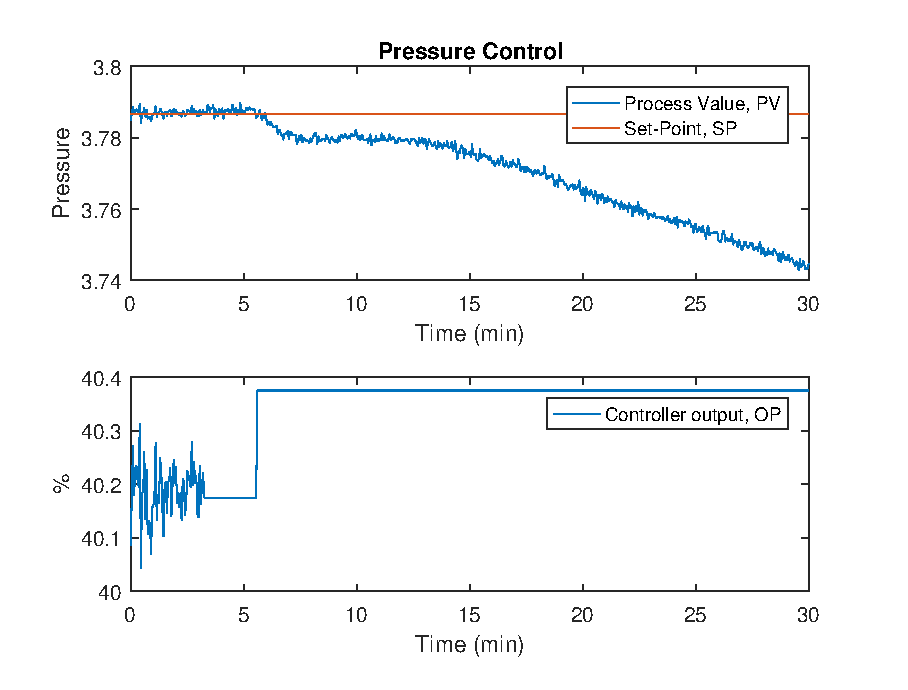
\includegraphics[width=0.85\textwidth]{fig/tuning/PC1024_simc.eps}
	\caption{Response of the controller \texttt{PC\_1024} when applying a step on input}
	\label{fig:pc1024_simc}
\end{figure}
\begin{figure}[ht!]
	\centering
	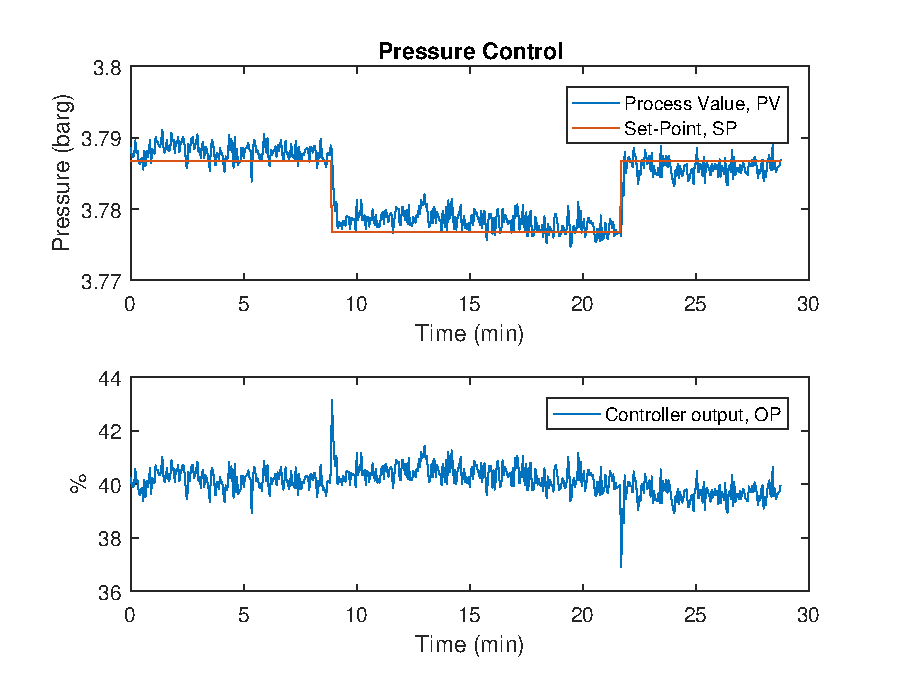
\includegraphics[width=0.85\textwidth]{fig/tuning/PC1024_tuned.eps}
	\caption{Response of the pressure controller \texttt{PC\_1024} after tuning and applying a step in the reference value}
	\label{fig:pc1024_tuned}
\end{figure}

\subsection{Tuning of \texttt{24\_FC1015}}
When it came to the controller \texttt{24\_FC1015}, I came to the conclusion that all responses were unstable when trying to use the classic tuning methods. I therefore went back to the even more classic method of trial and error. By tweaking $K_p$ and $T_i$ within reasonable limits we hit a set of parameters, $K_p = 0.2$ and $T_i = 5$, which gave fairly good response. This is shown in \autoref{fig:fc1015_tuned}. We see that the process value follows the reference pretty good.

\begin{figure}[ht!]
	\centering
	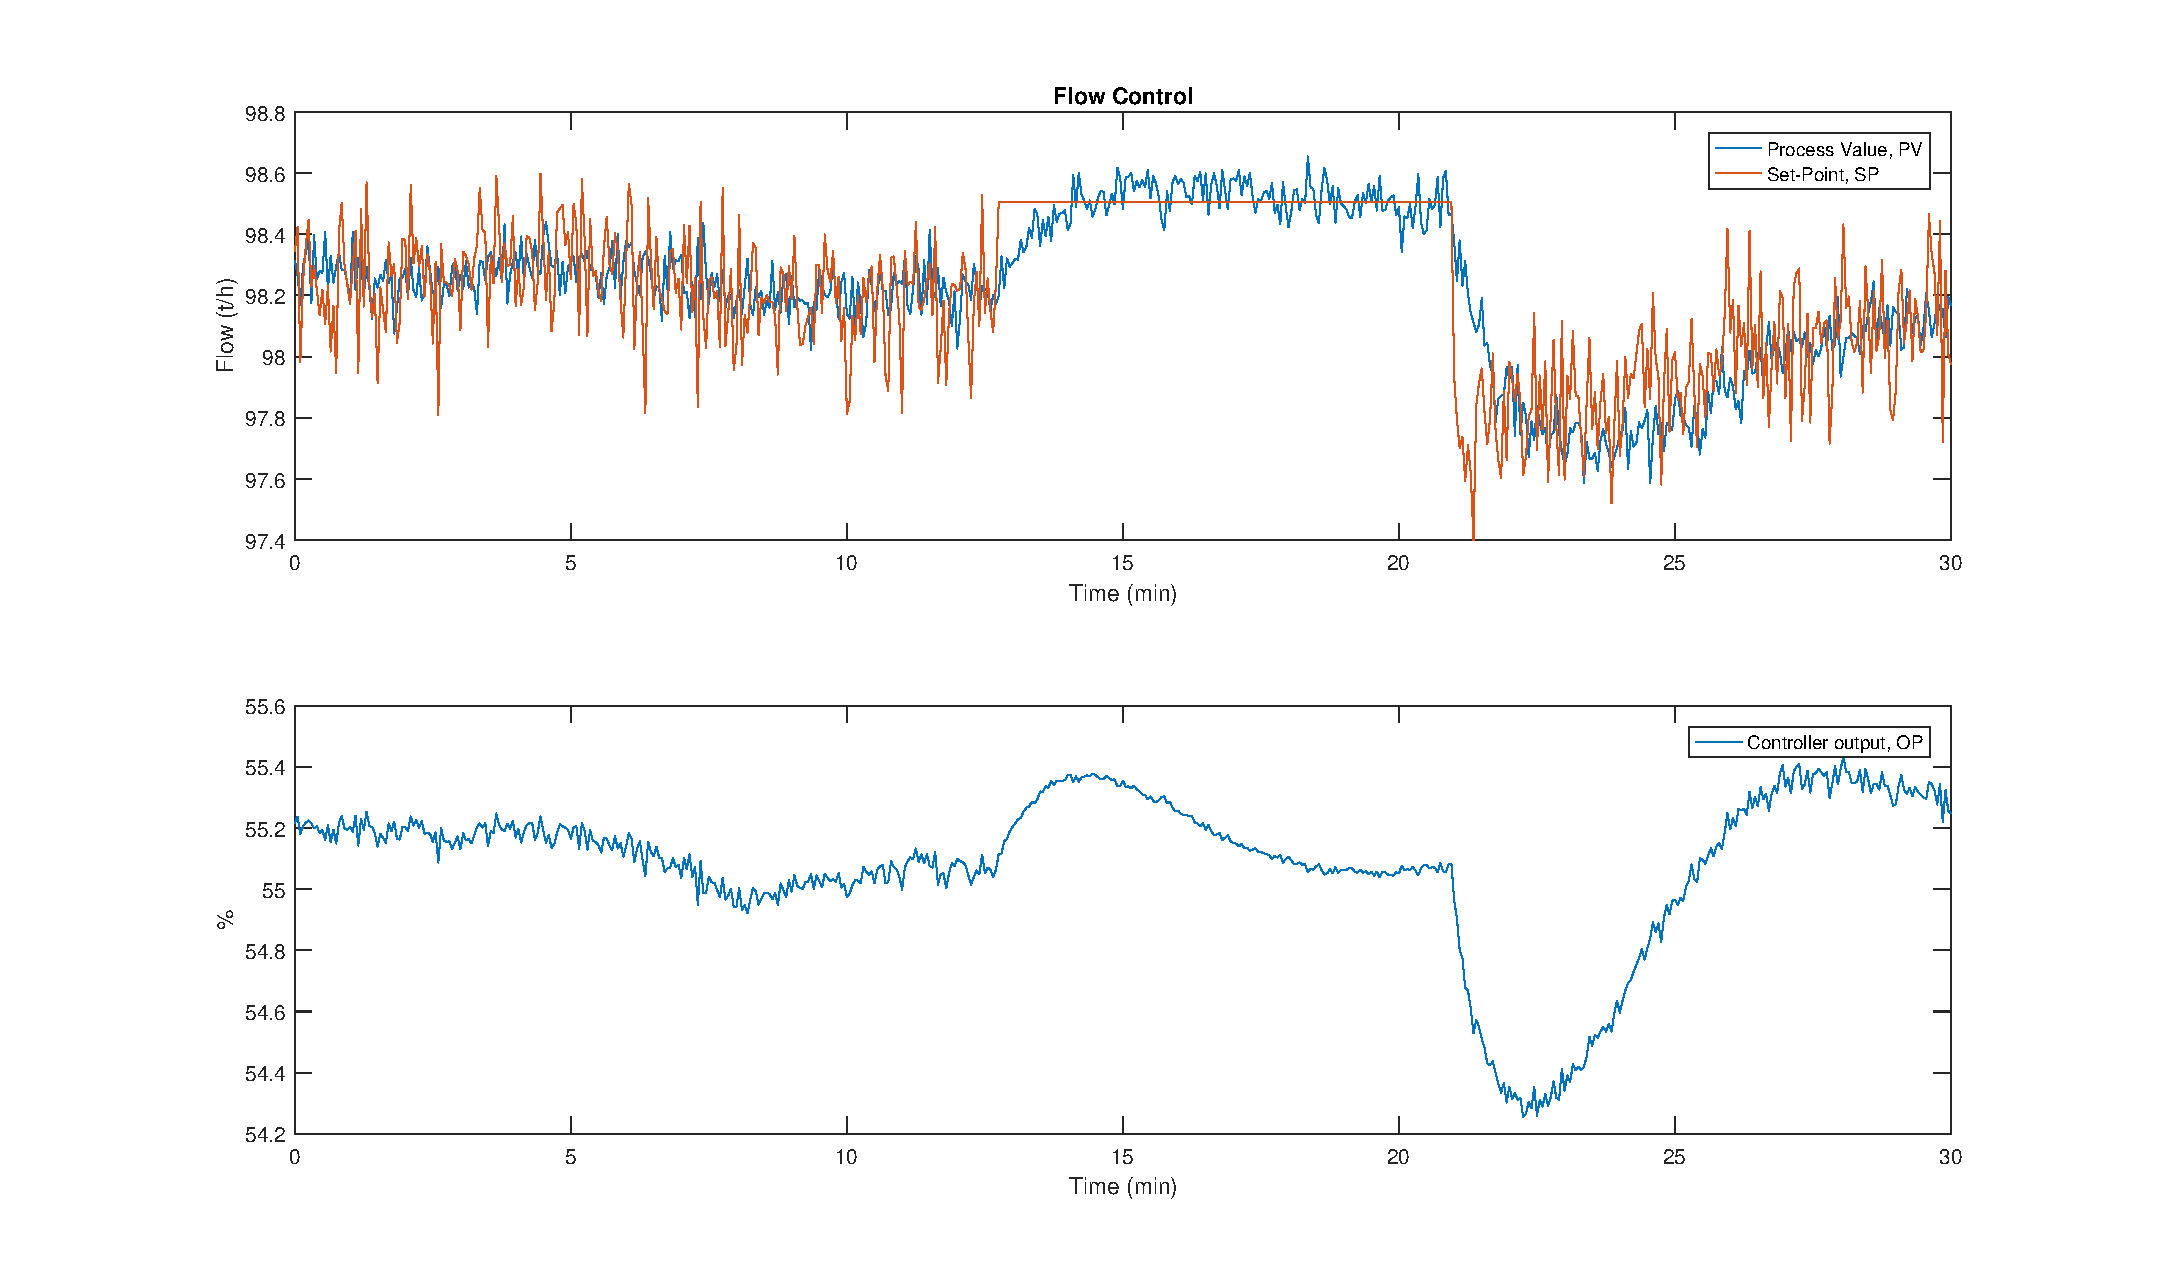
\includegraphics[width=0.85\textwidth]{fig/tuning/FC1015_tuned.eps}
	\caption{Response of the controller \texttt{24\_FC1015} after tuning using trial and error}
	\label{fig:fc1015_tuned}
\end{figure}

\clearpage
\section{Tuning and identification of level controllers}\label{sec:levelcontrollers}
We now move on to the identification and tuning of the level controllers \texttt{24\_LC1015} and \texttt{24\_LC1016}. This will be done by changing the setpoints of the controllers such that the manipulated variables are excited. The base code for this is shown in \autoref{lst:identification}, where minor adjustments is done to the .txt-file we import based on what data we have exported from K-Spice and which contoller we have excited.

\subsection{Level controller \texttt{24\_LC1016}}\label{ssec:lc1016}
We start by doing an set point exciting experiment on the controller \texttt{24\_LC1016}, where we do several step changes in the set point, and then observe the output. We then import this to MATLAB and use the built in function \mcode{n4sid} to estimate a state space realization of the system we are looking at. The general code to do this is shown in \autoref{lst:identification} in \autoref{ch:matlab}. In \autoref{fig:lc1016_identified} we see the actual response of the controller  normalized and compared to the identified model. We see that the identified model is fairly good. 

\begin{figure}[ht!]
	\centering
	\includegraphics[width=0.8\textwidth]{fig/identification/lc1016_order2_ref.eps}
	\caption{Actual response and response of identified model of order 2 for the controller \texttt{24\_LC1016}}
	\label{fig:lc1016_identified}
\end{figure}

Using this model we get the second order discrete time system system
\begin{equation}
	\begin{aligned}
		x_{n+1} &= \underbrace{\begin{bmatrix}
			1.001 & 0.02635 \\ -0.009939 & 0.1251
		\end{bmatrix}}_{A} x_n +
		\underbrace{\begin{bmatrix}
			-7.587\cdot 10^{-5} \\ -0.006211
		\end{bmatrix}}_{B} u_n \\
		y_n &= \underbrace{\begin{bmatrix}
			19.36 & -0.6743
		\end{bmatrix}}_{C} x_n + 
		\underbrace{0}_{D} u
	\end{aligned}
\end{equation}
which yields the step response shown in \autoref{fig:lc1016_untuned}, where we see that we have a somewhat underdamped system.

\begin{figure}[ht!]
	\centering
	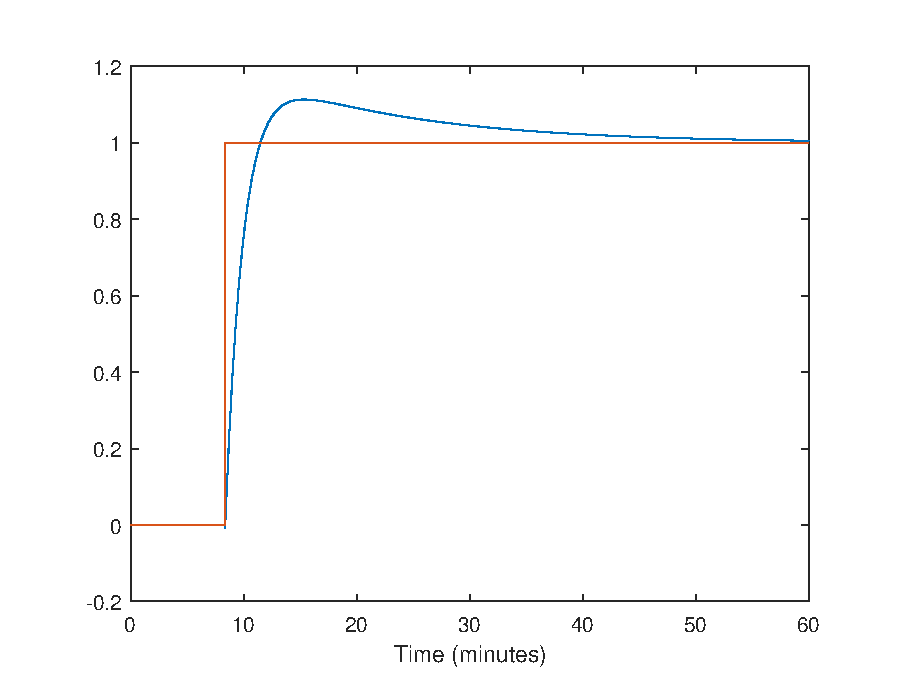
\includegraphics[width=0.8\textwidth]{fig/identification/lc1016_simulation_untuned.eps}
	\caption{Step response of the controller \texttt{24\_LC1016} for identified model before tuning}
	\label{fig:lc1016_untuned}
\end{figure}

However, tuning the parameters of the controller does not give severly increased response. Anyway, with $T_i = \SI{750}{\second}$ and $K_p = -4$ in MATLAB we get the slightly faster response and faster approach to the stationary value. Using gain scaling as shown in \autoref{eq:scaling} we get the scaling and gain parameters

\begin{equation}
	\begin{aligned}
		G &= \frac{u_{\text{exp}}}{u_{\text{meas}}} = \frac{4}{-4.83} = -0.83\\
		K_p &= GK_{p, \text{MATLAB}} = -0.83\cdot(-4) = 3.32\\
		T_i &= 750
	\end{aligned}
\end{equation}

Applying these parameters and running the MCL-script given in \autoref{lst:lc1016_tuned} in \autoref{ch:mcl} we get the response shown in \autoref{fig:lc1016_tuned}. Here we see that the response is pretty fast and accurate, but we also see anomalies in the start and end of the plot. This is due to the fact that the main composition controllers are put in manual mode after five minutes of the simulation, and back again to automatic mode after 115 minutes, so that the tuning of this level controller is to be more precise. When returning to automatic mode, the temperature controller \texttt{24\_TC1015} looks to decrease the reflux flow into the chamber which again leads to less flow out of the drum where we try to control the level. Because of this what we care about here is the response between five and 115 minutes, which we see is pretty good.

\begin{figure}[ht!]
	\centering
	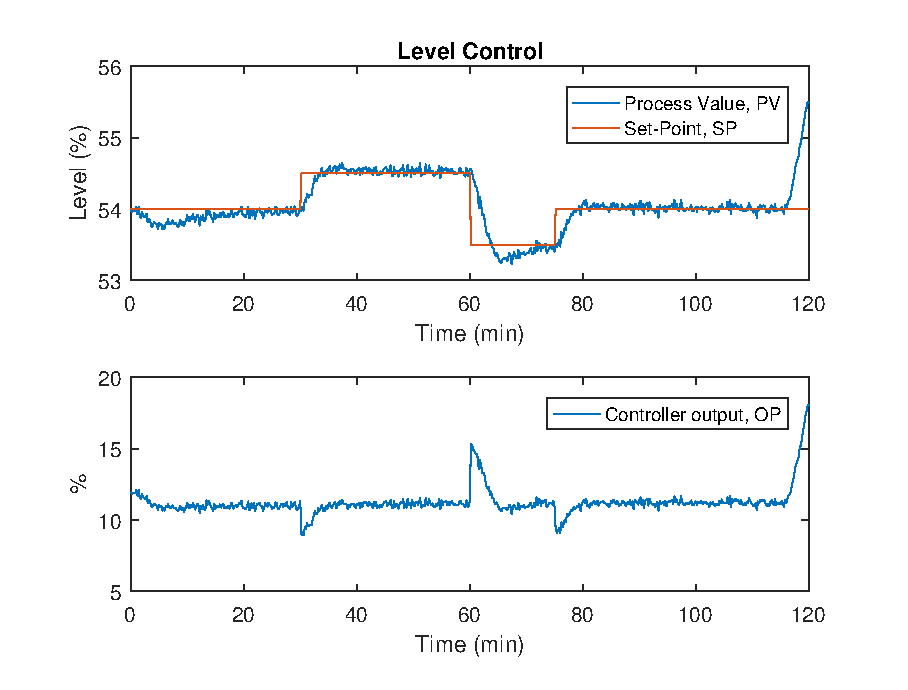
\includegraphics[width=0.95\textwidth]{fig/identification/lc1016_tuned.eps}
	\caption{Tuned response of the controller \texttt{24\_LC1016} when applying several step reference changes}
	\label{fig:lc1016_tuned}
\end{figure}

\subsection{Level controller \texttt{24\_LC1015}}
Now we move on to the level controller \texttt{24\_LC1015} which controls the liquid level of the distillation column. By performing a step change in the reference and simulating for five hours we get the response shown in \autoref{fig:lc1015_untuned}. Here we apply a step change of 1.5\% after 90 minutes and then simulate for another 210 minutes.

\begin{figure}[ht!]
	\centering
	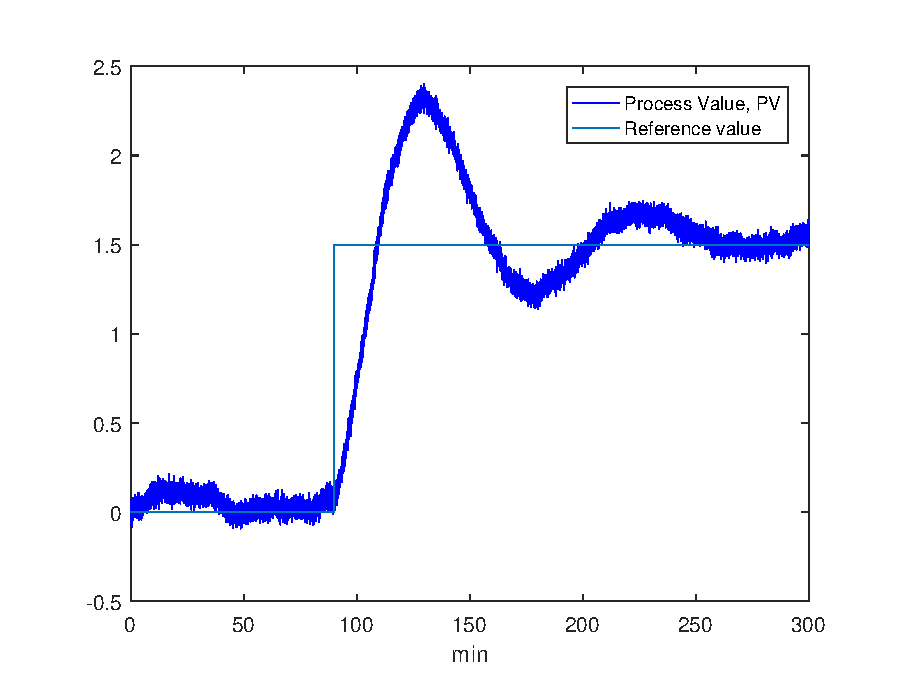
\includegraphics[width=0.95\textwidth]{fig/identification/lc1015_simulation_untuned.eps}
	\caption{Response of the controller \texttt{24\_LC1015} with step change after 90 minutes}
	\label{fig:lc1015_untuned}
\end{figure}

Further we fit a model using the same procedure as in \autoref{ssec:lc1016} and obtain the model 

\begin{equation}
	\begin{aligned}
		x_{n+1} &= x_n - 1.155\cdot 10^{-5} u_n \\
		y_n &= 179.03 x_n
	\end{aligned}
\end{equation}

This model fits very good with the obtained data, as shown in \autoref{fig:lc1015_identified}.

\begin{figure}[ht!]
	\centering
	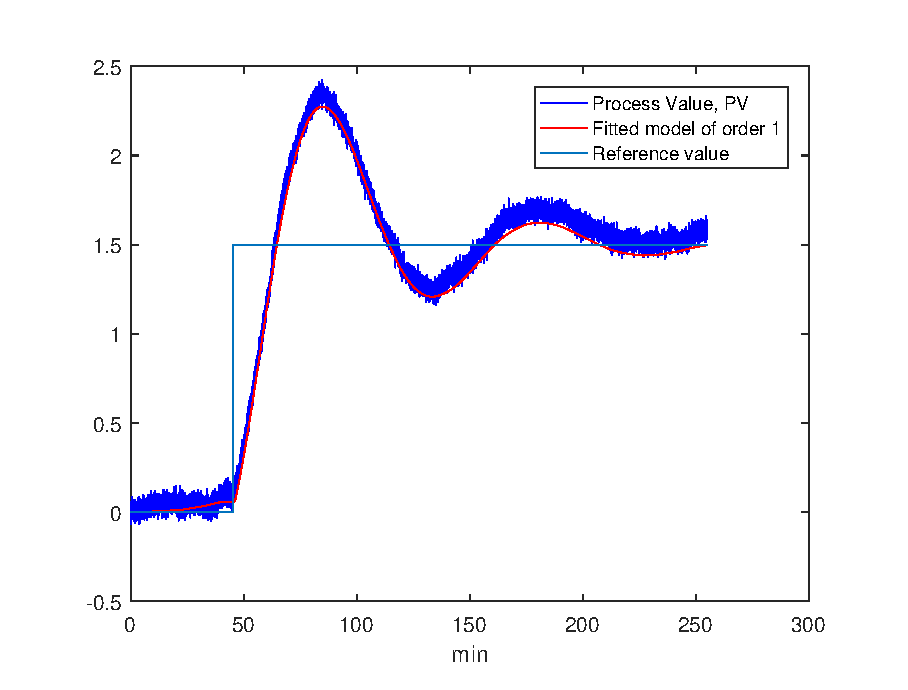
\includegraphics[width=0.95\textwidth]{fig/identification/lc1015_order1.eps}
	\caption{Fitted model and actual data for \texttt{24\_LC1015}}
	\label{fig:lc1015_identified}
\end{figure}

This fitted model is now used for tuning the controller. With the initial parameters $K_p = 1$ and $T_i = 500$ as we used when identifying the system, gives the response shown in \autoref{fig:lc1015_simulation_untuned}. Here we see an oscillating system which is not desirable.

\begin{figure}[ht!]
	\centering
	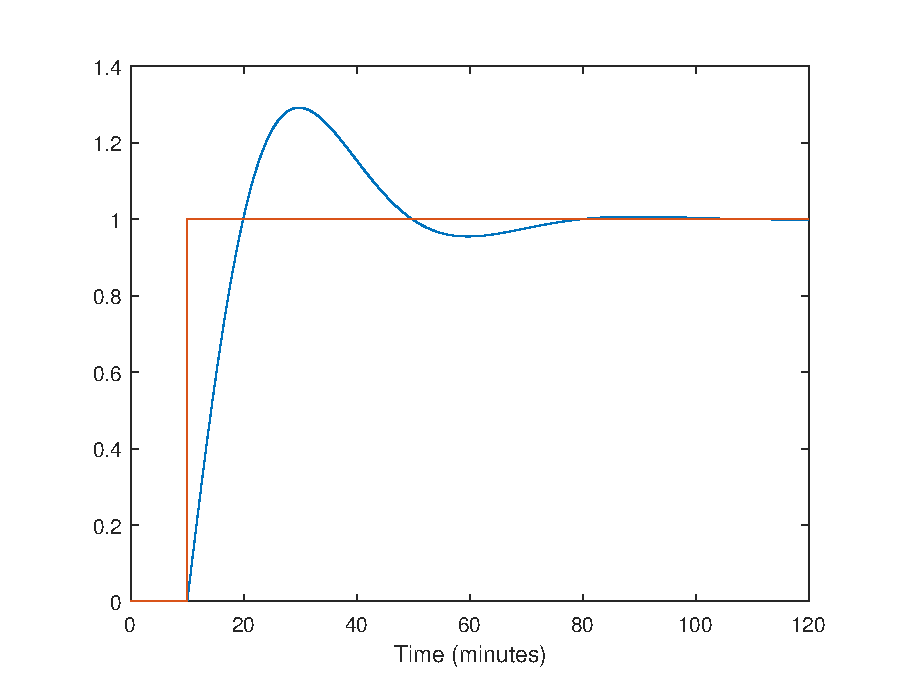
\includegraphics[width=0.95\textwidth]{fig/identification/lc1015_simulation_before.eps}
	\caption{Response of the model for the controller \texttt{24\_LC1015} with $K_p = 1$ and $T_i = 500$ before tuning}
	\label{fig:lc1015_simulation_untuned}
\end{figure}

Finding the internal scaling gain and tuning by som quick trial and error we find a good set of parameters given by

\begin{equation}
	\begin{aligned}
		G &= \frac{u_{\text{exp}}}{u_{\text{meas}}} = \frac{1}{-0.31} = -3.22 \\
		K_p &= GK_{p,\text{MATLAB}} = -3.22\cdot(-3) = 9.66\\
		T_i &= 1200
	\end{aligned}
\end{equation}
These parameters applied to the K-Spice model gives the performance shown in \autoref{fig:lc1015_tuned}. Here we have just a small overshoot and fast approach to steady state value, which is really good compared to before tuning as shown in \autoref{fig:lc1015_untuned}. 

\begin{figure}[ht!]
	\centering
	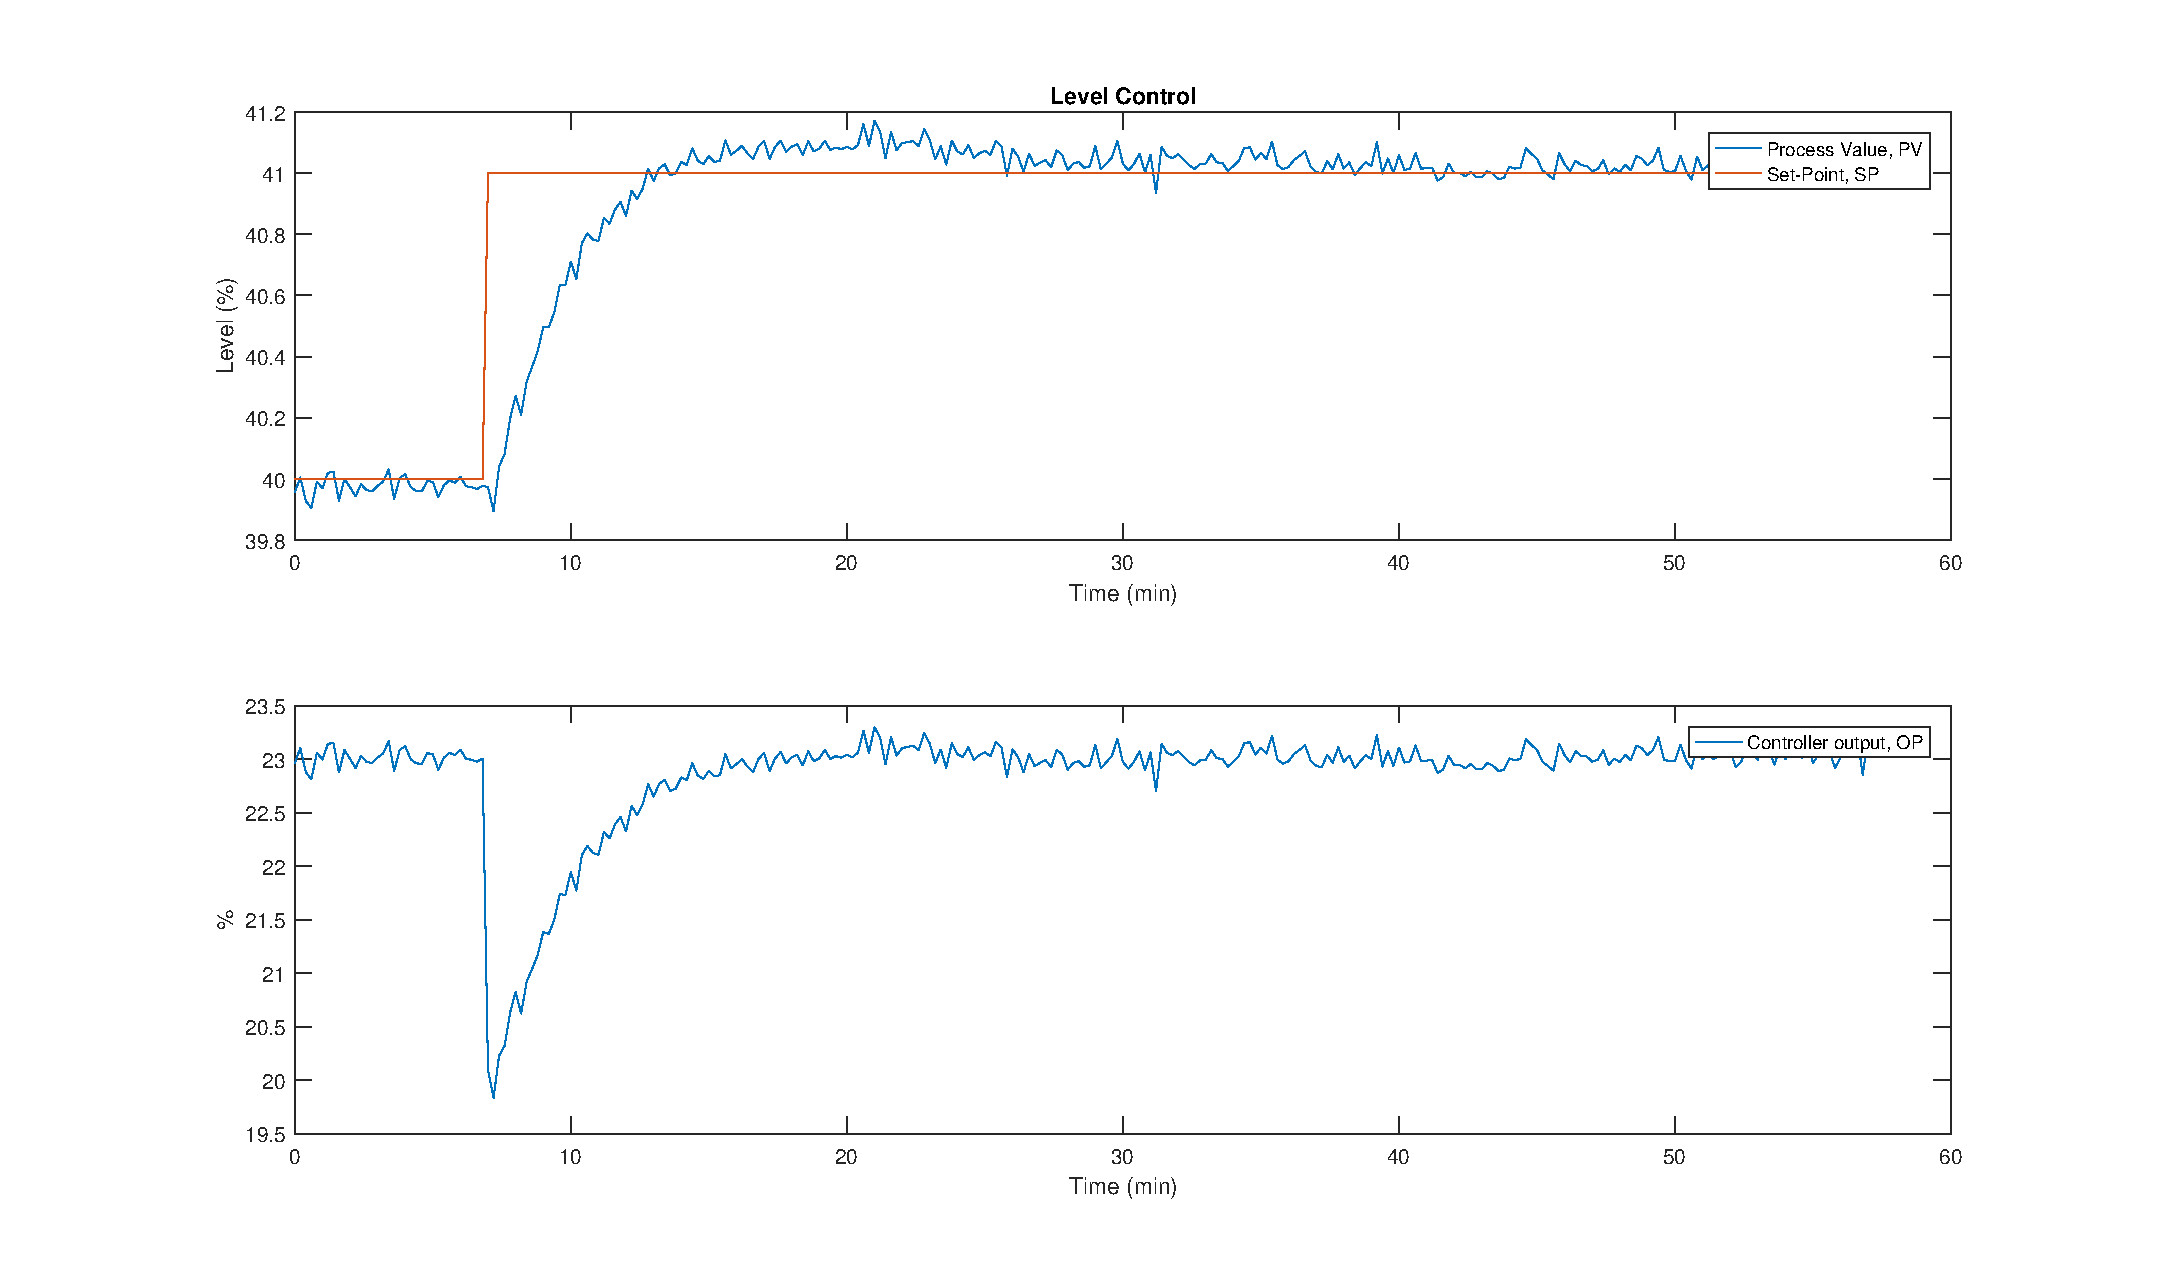
\includegraphics[width=0.95\textwidth]{fig/identification/lc1015_tuned.eps}
	\caption{Response of the controller  \texttt{24\_LC1015} after tuning}
	\label{fig:lc1015_tuned}
\end{figure}

\clearpage
\section{Identification and tuning of the composition controllers}
We now move on to two final controllers, namely the top level composition controllers. These controllers are temperature controllers that while operating makes sure the temperature in two trays in the distillation column is within acceptable regions such that the composition of what's inside the trays stays within their impurty-limits. Here we have \texttt{24\_TC1015} controlling tray 88 to a set temperature of \SI{35.30}{\degreeCelsius} while \texttt{24\_TC1088} controls the temperature in tray 19 to a set temperature of \SI{48.51}{\degreeCelsius}. The manipulated variables for the composition controllers can be excited directly, and that is what we aim to do.

\subsection{Identification and tuning of temperature controller \texttt{24\_TC1088}}
As mentioned this controller's task is to control the temperature in tray 19 such that there are maximum 2.5\% iso-butane in the column. This is achieved by keeping the temperature in the tray at \SI{48.51}{\degreeCelsius} which corresponds to 1.25\% iso-butane. To identify this system we use the script \autoref{lst:tc1088_exp} in \autoref{ch:mcl} doing several step changes in the controller output. As this is an integrating process we then get the process values shown in \autoref{fig:tc1088_exp}. Here we have also fitted a model of second order using the MATLAB script shown in \autoref{lst:identification}, with slight tweaks so that we use the right controller of course. This results in a good fit, which we see in \autoref{fig:tc1088_exp}. The modeled second order system can be described by the state space realization

\begin{equation}
	\begin{aligned}
		x_{n+1} &= \underbrace{\begin{bmatrix}
			0.9996 & 0.0292 \\ -0.0006 & -0.1474
		\end{bmatrix}}_{A} x_n +
		\underbrace{\begin{bmatrix}
			0.00002 \\ -0.0014
		\end{bmatrix}}_{B} u_n \\
		y_n &= \underbrace{\begin{bmatrix}
			16.1739 & -0.9862
		\end{bmatrix}}_{C} x_n + 
		\underbrace{0}_{D} u
	\end{aligned}
\end{equation}


\begin{figure}[ht!]
	\centering
	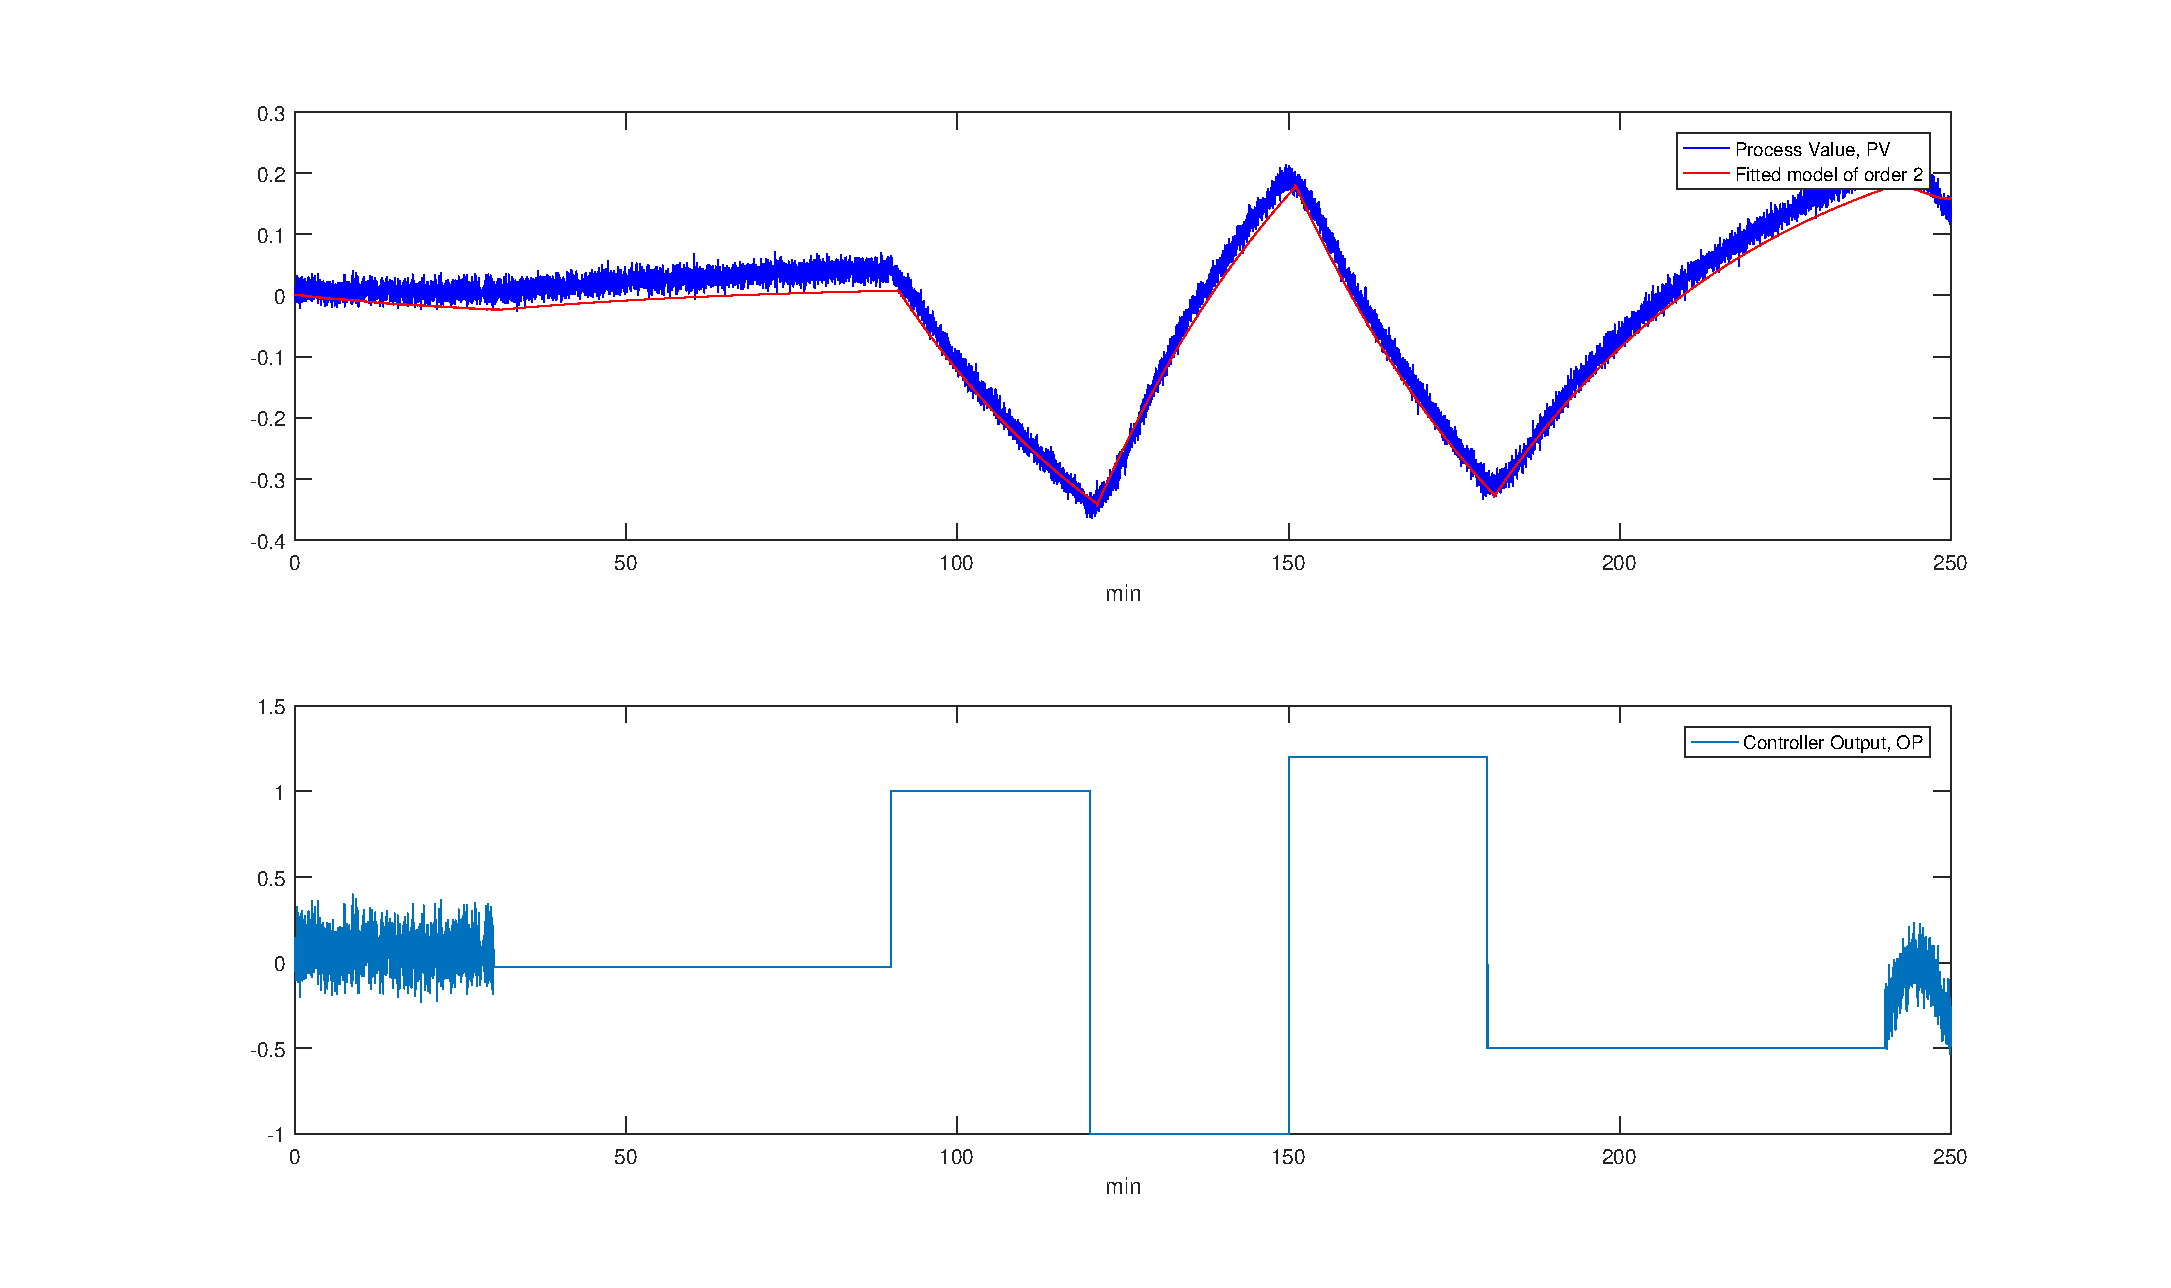
\includegraphics[width=0.95\textwidth]{fig/identification/tc1088_identify.eps}
	\caption{Process value, fitted model and controller output for \texttt{24\_TC1088} when running the experiment}
	\label{fig:tc1088_exp}
\end{figure}
\begin{figure}[ht!]
	\centering
	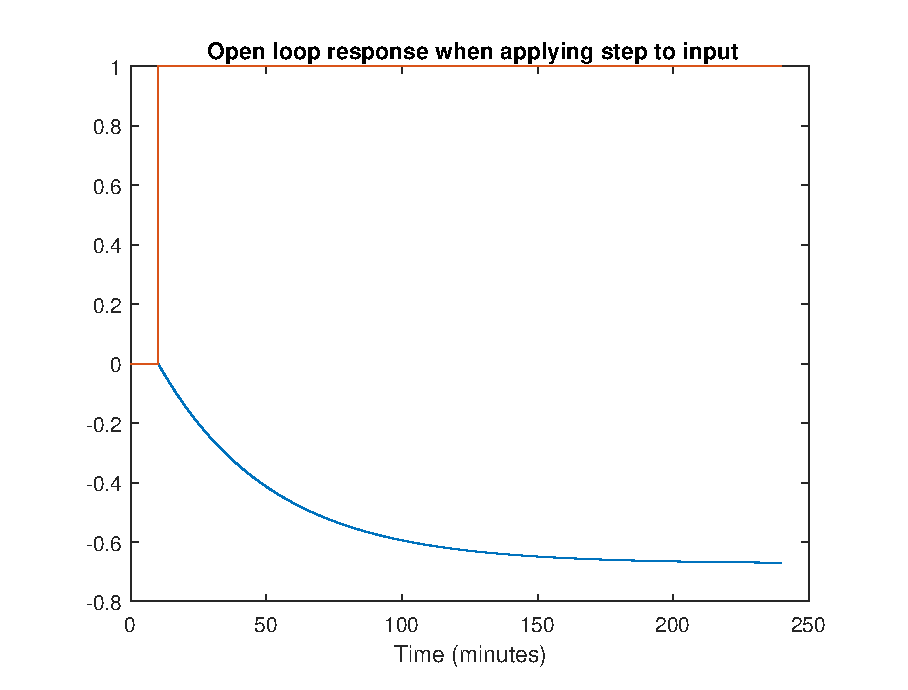
\includegraphics[width=0.95\textwidth]{fig/identification/tc1088_OL.eps}
	\caption{Open loop response of the fitted model when applying unit step to input}
	\label{fig:tc1088_OL}
\end{figure}

Tuning this controller we use SIMC-tuning as given in \autoref{eq:simc} and from \autoref{fig:tc1088_OL} we read off the parameters 

\begin{equation}
	\begin{aligned}
		y(\infty) &= -0.6696 \\
		\tau &= 2476 \\
		\theta &= 60
	\end{aligned}
\end{equation}
which gives
\begin{equation}
	\begin{aligned}
		k &= \frac{y(\infty)}{\Delta u } = -0.6696\\
		k' &= \frac{k}{\tau} = -2.704 \cdot 10^{-4}
	\end{aligned}
\end{equation}

Then using the rules for SIMC-tuning we get the set of parameters shown in \autoref{table:tc1088_parameters}.

\begin{table}[h]
	\caption{Set of parameters for different choices of $\tau_c$}
	\label{table:tc1088_parameters}
	\begin{center}
	\begin{tabular}{|c|c|c|}
	\hline
	$\tau_c$ & $K_c$ & $T_i$ \\
	\hline
	$\theta$ & $-30.8$ & $480$\\
	$3\theta$ & $-15.4$ & $960$\\
	$5\theta$ & $-10.3$ & $1440$\\
	\hline
	\end{tabular}
	\end{center}
\end{table}

Choosing $\tau_c = 5\theta$ we get the response shown in \autoref{fig:tc1088_tuned_model}, which is good. Before applying these parameters, we as earlier need to compensate for internal gain in the controller. Doing a step change to reference we get the values of internal gain and applied gain shown in \autoref{eq:tc1088_internal}, before we apply these parameters to the K-Spice simulation, and get the response shown in \autoref{fig:tc1088_tuned_kspice}. Here we see that the controller hits the reference value with good accuracy without overshooting, which when taking the purity constraints into consideration is a good thing. The response also reaches the setpoint fairly fast.

\begin{equation} \label{eq:tc1088_internal}
	\begin{aligned}
		G &= \frac{-2.5}{57.97 - 52.84} = -0.487\\
		\implies K_{p,\text{applied}} &= -10.3\cdot(-0.487) = 5.02
	\end{aligned}
\end{equation}

\begin{figure}[ht!]
	\centering
	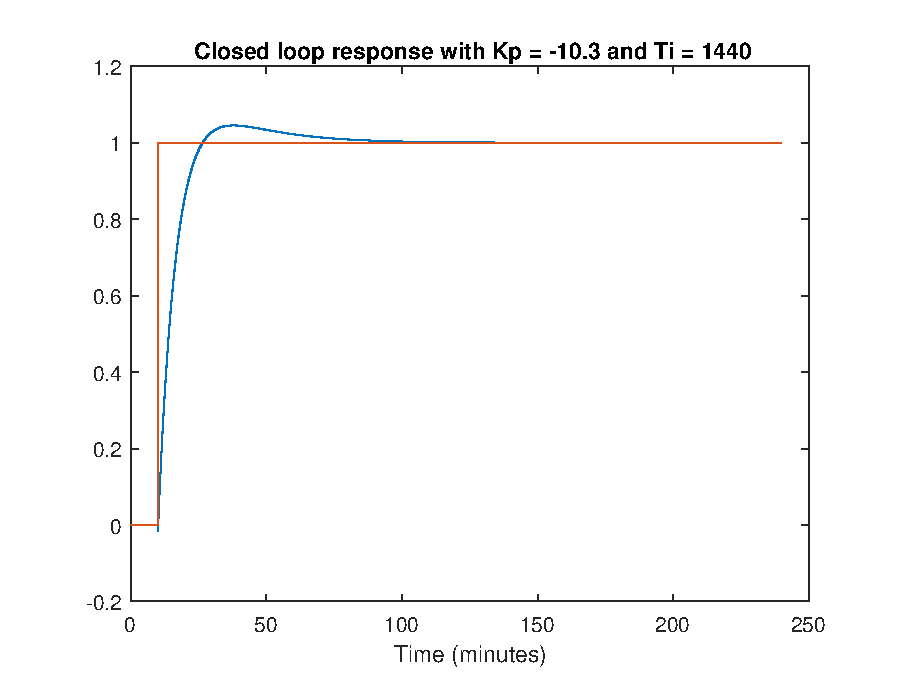
\includegraphics[width=0.95\textwidth]{fig/identification/tc1088_tuned.eps}
	\caption{Tuned response of the model with $K_p = -10.3$ and $T_i = 1440$}
	\label{fig:tc1088_tuned_model}
\end{figure}

\begin{figure}[ht!]
	\centering
	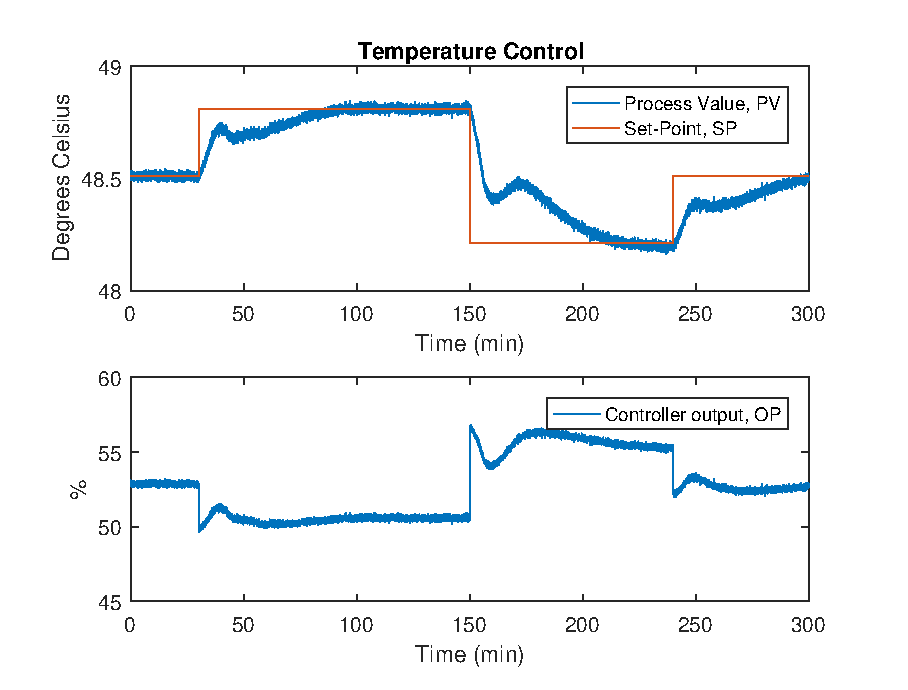
\includegraphics[width=0.95\textwidth]{fig/identification/tc1088_tuned_kspice.eps}
	\caption{Response of K-Spice simulation of \texttt{24\_TC1088} when applying steps to reference}
	\label{fig:tc1088_tuned_kspice}
\end{figure}

\clearpage
\subsection{Identification and tuning of temperature controller \texttt{24\_TC1015}}
We now move on to the final controller we are going to tune for now, namely the composition controller for the amount of n-butane in the top product. The maximum allowed impurity is specified to 4\%, which is achieved at \SI{35.85}{\degreeCelsius} in tray 88. To stay within this constraint we aim at controlling the temperature to the set point of \SI{35.3}{\degreeCelsius} which results in 2\% n-butane in the top product. Doing a similar experiment as for the previous controller we get the response shwen in \autoref{fig:tc1015_identify} and the identified second order state space model given by

\begin{equation}
	\begin{aligned}
		A &= \begin{bmatrix}
			1 & 0.0255 \\ 0.0008 & -0.0659
		\end{bmatrix} \\
		B &= \begin{bmatrix}
			-0.0072 \\ 0.1938
		\end{bmatrix} \cdot 10^{-3}\\
		C &= \begin{bmatrix}
			19.2362 & -0.9464
		\end{bmatrix}\\
		D &= 0
	\end{aligned}
\end{equation}

\begin{figure}[ht!]
	\centering
	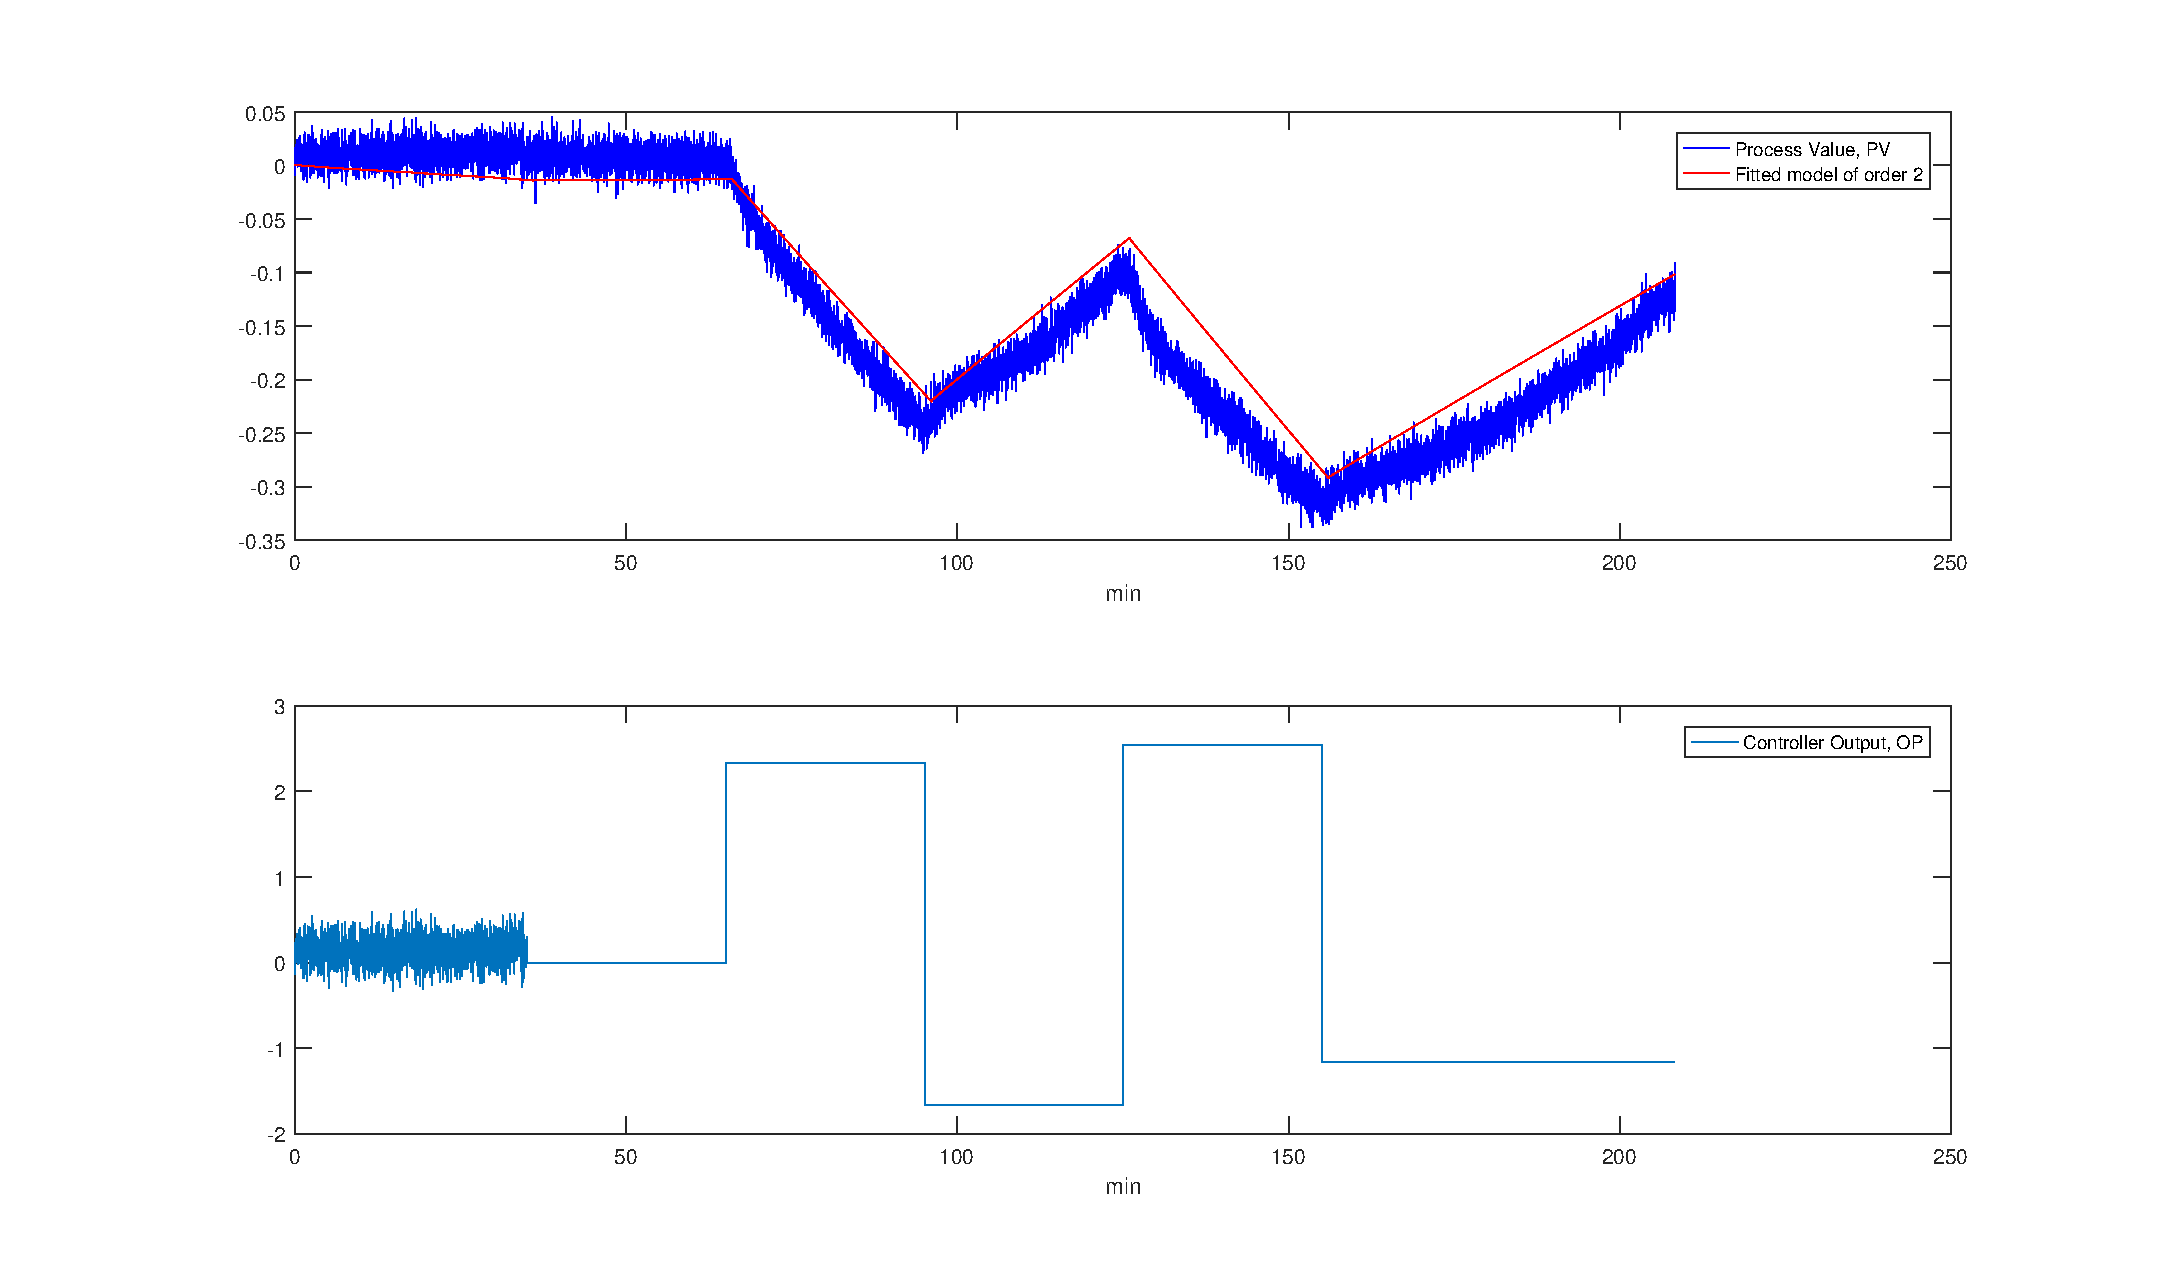
\includegraphics[width=0.95\textwidth]{fig/identification/tc1015_identify.eps}
	\caption{Response of \texttt{24\_TC1015} after several steps in controller output together with identified model of second order}
	\label{fig:tc1015_identify}
\end{figure}

Observing the open loop step response to this system we get the response shown in \autoref{fig:tc1015_OL}, which we see is an integrating response. Applying the SIMC-tuning method as in \autoref{eq:simc} to this output we get values
\begin{equation}
	\begin{aligned}
		k' &= \frac{\Delta y}{\Delta t \Delta u} = \frac{-0.2137-(-0.0201)}{(5000-4000)\cdot 1} \\
		&= -4.84\cdot 10^{-5}
	\end{aligned}
\end{equation}
which with different choices of $\tau_c$ for $\theta = \SI{60}{\second}$ gives the controller parameters table shown in \autoref{table:tc1015_parameters}.

\begin{table}[h]
	\caption{Set of parameters for different choices of $\tau_c$}
	\label{table:tc1015_parameters}
	\begin{center}
	\begin{tabular}{|c|c|c|}
	\hline
	$\tau_c$ & $K_c$ & $T_i$ \\
	\hline
	$\theta$ & $-452$ & $480$\\
	$3\theta$ & $-226$ & $960$\\
	$5\theta$ & $-150$ & $1440$\\
	$7\theta$ & $-113$ & $1920$\\
	\hline
	\end{tabular}
	\end{center}
\end{table}

\begin{figure}[ht!]
	\centering
	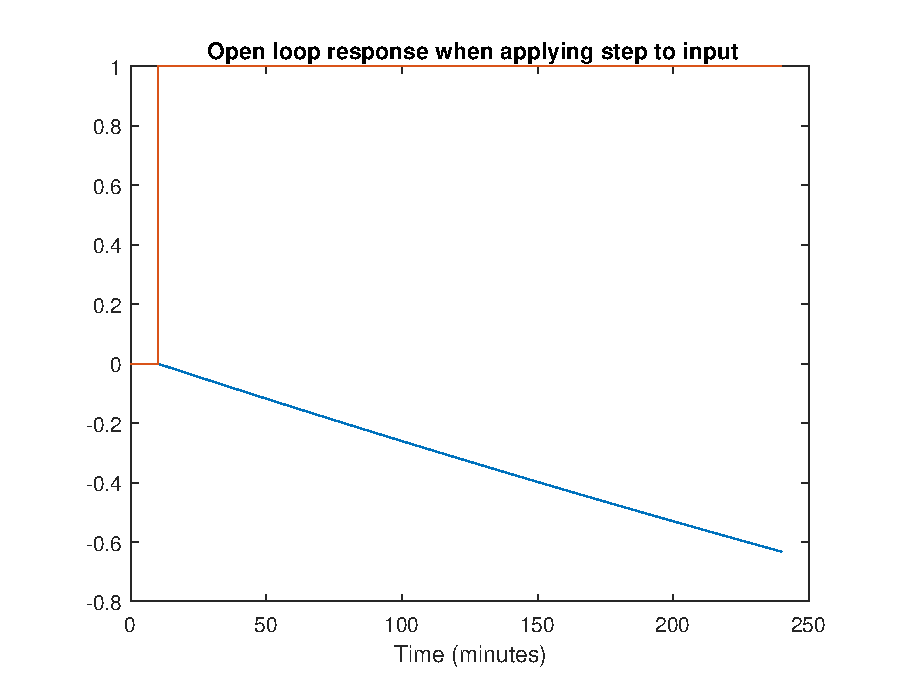
\includegraphics[width=0.95\textwidth]{fig/identification/tc1015_OL.eps}
	\caption{Open loop step response of \texttt{24\_TC1015}}
	\label{fig:tc1015_OL}
\end{figure}

We here get the best result when choosing $\tau_c = 5\theta$ which gives the step response shown in \autoref{fig:tc1015_tuned_model}. From here we need to find the internal gain factor, which by doing a step reference change as always are found to be $G = -0.44$. This means that $K_{p,\text{applied}} = 66$. The response is shown in \autoref{fig:tc1015_tuned}. Here we see fast approach to an increase in the temperature setpoint, but somewhat slower when we apply a decrease in reference temperature. All in al this system behaves reasonably good with this controller tuning.

\begin{figure}[ht!]
	\centering
	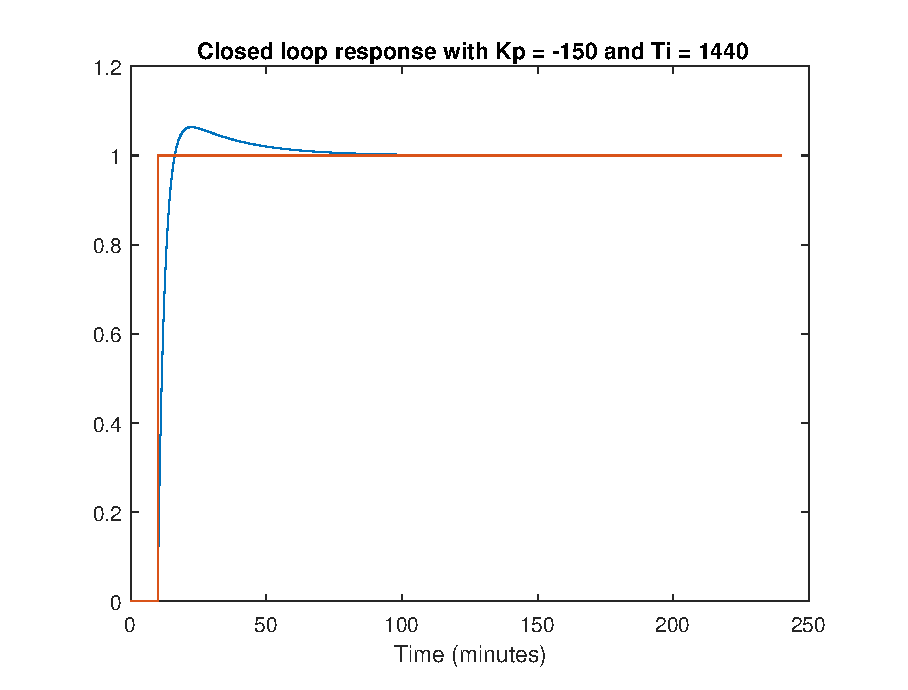
\includegraphics[width=0.95\textwidth]{fig/identification/tc1015_tuned_model.eps}
	\caption{Stop response of the tuned model of \texttt{24\_TC1015}}
	\label{fig:tc1015_tuned_model}
\end{figure}
\begin{figure}[ht!]
	\centering
	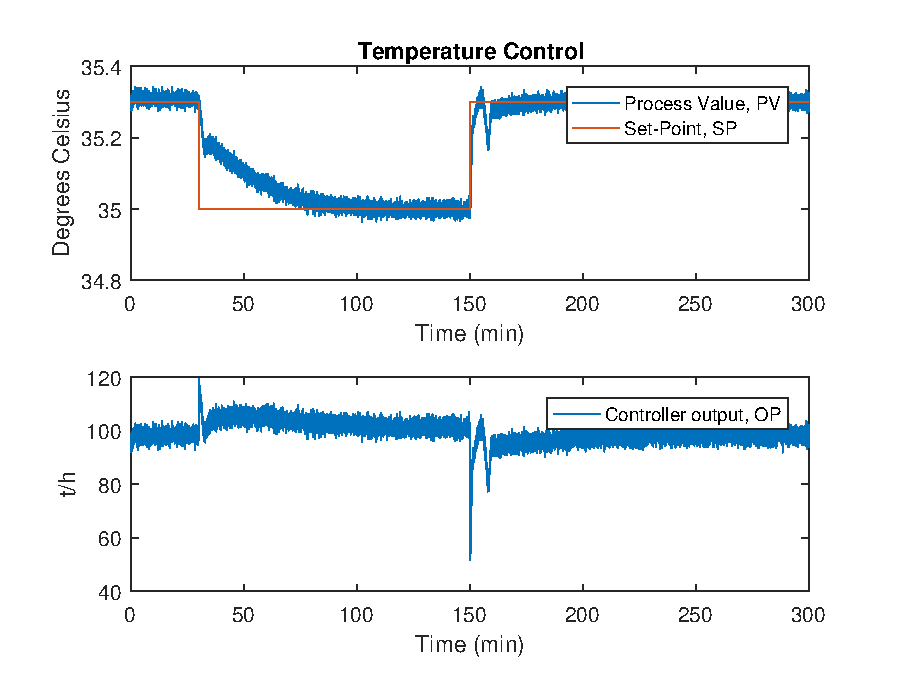
\includegraphics[width=0.95\textwidth]{fig/identification/tc1015_tuned_kspice.eps}
	\caption{Response of the controller \texttt{24\_TC1015} when doing step changes in reference temperature}
	\label{fig:tc1015_tuned}
\end{figure}